\documentclass[12pt,a4paper]{article}
\usepackage[utf8]{inputenc} %polskie znaki
\usepackage[T1]{fontenc}	%polskie znaki
\usepackage{amsmath}		%matematyczne znaczki :3
\usepackage{enumerate}		%Dodatkowe opcje do funkcji enumerate
\usepackage{geometry} 		%Ustawianie marginesow
\usepackage{graphicx}		%Grafika
\usepackage{wrapfig}		%Grafika obok textu
\usepackage{float}			%Allows H in figure
\usepackage{hyperref}		%Allows hyperlinks
%\pagestyle{empty} 			%usuwa nr strony
\usepackage{todonotes}		%Todo notatki
\usepackage{lipsum}         %Lorem text
\usepackage{ntheorem}   	% for theorem-like environments
\usepackage{mdframed}   	% for framing
\usepackage{subcaption}		% subfigure (image placing)
\usepackage{pdfcomment}		% Komentarze (z bazowego pdf'a)
\usepackage{xparse}			% New commands with optional arguments
\usepackage{ifthen}			% If then - funkcje!
\usepackage{expl3}			% Deklarowanie zmiennych
\usepackage{pgf}			% Aktualne rachunki \pgfmathparse{}
\usepackage{amsmath} 		% For mathematical symbols and structures
\usepackage{amsfonts}		% Zbiór liczb naturalnych + formatowanie
\usepackage{ulem}			% Przekreślony text
%\usepackage[colorlinks=true, linkcolor=blue, urlcolor=red, citecolor=green]{hyperref}
\usepackage{fontawesome5}
\usepackage{mathtools}
%\usepackage{multirow} 		% Required for merging rows
\newcommand{\niton}{\not\owns}

\newgeometry{tmargin=2cm, bmargin=2cm, lmargin=2cm, rmargin=2cm} 

%Counter commands{
	\newcounter{definicja}
	\setcounter{definicja}{1} 
	\newcounter{twierdzenie}
	\setcounter{twierdzenie}{1} 
	\newcounter{przyklady}
	\setcounter{przyklady}{1} 
	\newcounter{wnioski}
	\setcounter{wnioski}{1} 
	
	\newcommand{\counter}[1]{
		\arabic{#1} \stepcounter{#1} 
	}
	\newcommand{\counterreset}[1]{\setcounter{#1}{1}}
	%}

%Define styles{
	\theoremstyle{break}
	\theoreminframepreskip{0.5cm}
	\theoremheaderfont{\bfseries}
	\newmdtheoremenv[%
	linecolor=white,%
	innertopmargin=\topskip,
	shadowsize=0,%
	innertopmargin=5,%
	innerbottommargin=5,%
	leftmargin=10,%
	rightmargin=10,%
	backgroundcolor=white!20,%
	innertopmargin=0pt,%
	ntheorem]{zad}{Zadanie}
	
	\mdfdefinestyle{zadanie}{
		linecolor=white,%
		innertopmargin=5,%
		innerbottommargin=5,%
		leftmargin=0,%
		rightmargin=0,%
		backgroundcolor=lightgray!20,%
		innertopmargin=8,
		innerbottommargin=8,
		skipabove = 5,
	}
	\mdfdefinestyle{wzor}{
		linecolor=cyan,%
		linewidth=2pt,%
		innertopmargin=0,
		innerbottommargin=8,
		leftmargin=10,%
		rightmargin=10,%
		backgroundcolor = white, 
		fontcolor = black,
		skipabove = 5,
		skipbelow = 5,
	}
	%}

%Zadania templatex%{
	\newcommand{\Obramowka}[1]{
		\begin{mdframed}[style=wzor]
			\centering #1
		\end{mdframed}
	}
	\newcommand{\Komentarz}[1]{
		\begin{mdframed}[style=zadanie]
			\textbf{Komentarz}\\
			#1
		\end{mdframed}
	}
	
	\newcommand{\Odp}[1]{
		\begin{mdframed}[style=zadanie]
			\textbf{Odpowiedź}\\
			#1
		\end{mdframed}
	}
	
	%}

% Set spacing before and after theorems
\setlength{\theorempreskipamount}{20pt}  % Space above the theorem
\setlength{\theorempostskipamount}{20pt} % Space below the theorem

\newtheorem{definition}{Definicja}[section]

\newtheorem{theorem}{Twierdzenie}[section]
\newtheorem{lemma}{Lemat}[section]
\newtheorem{wniosek}{Wniosek}[theorem]
\newtheorem{example}{Przykład}[section]
\newtheorem{exercise}{Ćwiczenie}[section]
\newtheorem{stwierdzenie}{Stwierdzenie}[section]
\newtheorem{obserwacja}{Obserwacja}[section]


\newcommand{\tg}{\text{tg}}
\newcommand{\ctg}{\text{ctg}}
\newcommand{\arctg}{\text{arctg}}
\newcommand{\arcctg}{\text{arcctg}}
\newcommand{\witw}{$\Leftrightarrow$}
\newcommand{\wynika}{$\Rightarrow$}
\newcommand{\UkladRownan}[2]{
	\left\{
	\begin{array}{l}
		#1 \\
		#2
	\end{array}
	\right.
}

\begin{document}
	\begin{enumerate}[1.]
	\item Kto jest autorem słów „Wszystko jest liczbą”, a kto „Liczby naturalne stworzył dobry Bóg, a reszta jest dziełem człowieka”?
	\Odp{
	"Wszystko jest liczbą" $\sim$ hasło Pitagorejczycy (Pitagoras z Samos) VI w. p.n.e.
	
	"Liczby naturalne stworzył dobry Bóg, a reszta jest dziełem człowieka" $\sim$ Leopold Kroneker
	}
	
	\item Czy zero jest liczbą naturalną? Podać argument za tym, by zaliczyć je do liczb naturalnych oraz za tym, by liczby naturalne zaczynać od jedynki.
	\Odp{
		Obie sytuacje są poprawne. 
		Za $0\in\mathbb{N}$: 
		\begin{itemize}
			\item konstrukcja zbioru liczb naturalnych na bazie zbiorów
			\item istnienie elementu neutralnego względem dodawania
			\item \textcolor{red}{TODO - Szukam argumenty}
		\end{itemize}
		
		Przeciw $0\in\mathbb{N}$:
		\begin{itemize}
			\item wzór na średnią, $n=0$ nie może być w mianowniku
			\item aksjomatyka Peano zaczyna się od 1
			\item Liczby rzymskie nie mają zapisu zera
			\item Brak problemu z dzieleniem przez liczby naturalne
			\item Coraz częściej jest używany zwrot "dodatnie liczby całkowite"
			\item 0 nie posiada rozkładu na czynniki pierwsze
		\end{itemize}
	}
	
	\item Podać definicję grupy.
	\Odp{
	$(G,*) \:: * \:: G \times G \longrightarrow G$
	\begin{enumerate}[1)]
		\item $\forall_{a,b,c \in G} \;(a*b)*c = a*(b*c)$ (łączność)
		\item $\exists_{e\in G} \; \forall_{a\in G} \; e*a=a*e=a$ (istnieje element neutralny)
		\item $\forall_{a\in G} \; \exists_{b\in G} \; a*b=b*a=e$ (istnieje element przeciwny)
	\end{enumerate}
	}
	
	\item Wytłumaczyć rolę klas równoważności w relacji równoważności.
	\Odp{
	Klasy równoważności w relacji równoważności odgrywają kluczową rolę, ponieważ każda relacja równoważności dzieli zbiór na rozłączne klasy, gdzie elementy w danej klasie są równoważne
	}
	\newpage
	\item Podać formalną definicję liczb całkowitych (na bazie liczb naturalnych).
	\Odp{
	$\mathbb{Z}=\frac{\mathbb{N}\times\mathbb{N}}{\sim} \qquad$
	$(m,n)\sim (a,b) \Leftrightarrow m+b = n+a$\\
	$(2,5)\sim (1,4)$, bo $2+4=5+1$ lub $2-5=1-4=-3$
	}
	
	\item Podać uzasadnienie tego, że przyjmujemy, iż $(-a)\cdot(-b) = ab$, nie zaś $(-a)\cdot(-b) = -ab$ dla $a, b \in \mathbb{N}$.
	\Odp{
	$(-2)(-5)=-10$\\
	$(-2)(10-5)=-2\cdot10+(-2)(-5)$\\
	$-2\cdot5=-10$ oraz $=-20+(-10)=-30$
	}
	
	\item Podać definicję pierścienia, pierścienia z jedynką.
	\Odp{
		\textbf{Pierścień}\\
		$(R,+,\cdot,0), \quad R\neq\emptyset$
		\begin{enumerate}[a)]
			\item $\forall_{a,b,c\in R}\; a+(b+c)=(a+b)+c$ (łączność dodawania)
			\item $\forall_{a\in R}\; a+0=a$ (element neutralny względem $+$)
			\item $\forall_{a\in R} \exists_{b\in R}\; a+b=0$ (istnienie elementu przeciwnego $b=-a$ względem dodawania)
			\item $\forall_{a,b\in R}\; a+b=b+a$ (grupa abelowa dodawania)
			\item $\forall_{a,b,c\in R} a\cdot(b\cdot c)=(a\cdot b)\cdot c$ (łączność mnożenia)
			\item $\forall_{a,b,c\in R} \; a\cdot(b+c)=(a\cdot b)+ (a\cdot c)$ (prawo rozdzielności)
			\item $\forall_{a,b,c\in R} \; (b+c)\cdot a= (b\cdot a) + (c\cdot a)$ (prawo rozdzielności)
		\end{enumerate}
		
		\textbf{Pierścień z jedynką}\\
		$\exists_{1\in R} \forall_{a\in\mathbb{R}} a\cdot1=1\cdot a=a$
	}
	
	\item Podać definicję dzielników zera.
	\Odp{
		Element $a$ pewnego pierścienia, dla którego istnieje taki element $b$, że $ab=0$ oraz $b\neq 0$.
	}
	
	\item Podać formalną definicję liczb wymiernych (na bazie liczb całkowitych). Jakiej struktury jest to szczególny przypadek?
	\Odp{
	$\frac{\mathbb{Z}\times (\mathbb{Z}\setminus\emptyset)}{\sim} \qquad (m,n)\sim (a,b) \Leftrightarrow m\cdot b=n\cdot a$\\
	$\frac{m}{n}=\frac{a}{b}$ np. $(3,7)=(-6,-14)=\frac{3}{7}$
	}
	
	\item Podać „szkolną” definicję liczby wymiernej.
	\Odp{
		$p-$wymierna $\Leftrightarrow$ gdy można ją przedstawić w postaci ułamka o liczniku i mianowniku całkowitym.
	}
	\newpage
	\item Kto to był Nicolas Bourbaki?
	\Odp{
		To była grupa młodych matematyków, których celem było napisanie kompletu aktualnych podręczników do matematyki.
	}
	
	\item Zdefiniować „złoty podział”. Obliczyć liczbę otrzymaną w wyniku złotego podziału.
	\Odp{Złoty podział jest to podział pewnego odcinka w następujący sposób
	$$\frac{a}{b}=\frac{a+b}{a}$$, dla $a=1$
	$\frac{1}{b}=\frac{b+a}{1}$
	$b(b+1)=1$
	$b*2+b-1=0$
	$\Delta=1+4=5$
	$b_1=\frac{-1-\sqrt{5}}{2}$
	$b_2\frac{-1+\sqrt{5}}{2}$
	dotyczył on w szczególności pentagramu
	$$\frac{\text{duży}}{\text{średni}}=\frac{\text{średni}}{\text{mały}}$$
	}
	
	\item Udowodnić, że $\sqrt{2}$ nie jest liczbą wymierną.
	\Odp{
		Niech $\sqrt{2}$ będzie liczbą wymierną, można ją zatem zapisać w postaci 
		$$\sqrt{2}=\frac{a}{b} \Leftrightarrow 2=\frac{a^2}{b^2} \Leftrightarrow 2b^2=a^2$$
		Rozważmy przypadki 
		\begin{enumerate}[1$^\circ$]
			\item $a$ i $b$ nieparzyste - dostajemy natychmiast sprzeczność
			\item $a$ nieparzyste i $b$ parzyste - również otrzymujemy sprzeczność
			\item $a$ parzyste i $b$ nieparzyste - zatem możemy zapisać $a=2k$ otrzymujemy
			$$2b^2=4k^2$$
			$$b^2=2k^2$$
			Ponieważ prawa strona równania jest parzysta, to $b$ musi być parzyste - sprzeczność
			Sytuacja, że $a$ i $b$ są parzyste nie może zajść z konstrukcji liczb wymiernych.
			
		\end{enumerate}
	}
	\newpage
	\item Podać definicję ciała.
	\Odp{
		Ciało $\mathbb{K}$ to struktura $(\mathbb{K},+,\cdot,0,1)$ z działaniami odpowiednio $+$ i $\cdot$ (dodawanie i mnożenie) o własnościach 
		\begin{enumerate}[1)]
			\item $\forall_{a,b,c\in \mathbb{K}} a+(b+c)=(a+b)+c$ (łączność dodawania)
			\item $\forall_{a,b\in \mathbb{K}} a+b = b+a$ (przemienniość dodawania)
			\item $\forall_{a\in \mathbb{K}} a+0=a$ (istnienie zera)
			\item $\forall_{a\in\mathbb{K}} \exists_{b\in \mathbb{K}} : a+b=0$ (itnienie elementu przeciwnego)
			\item $\forall_{a,b,c\in \mathbb{K}} a\cdot (b\cdot c) = (a\cdot b)\cdot c$ (łączność mnożenia)
			\item $\forall_{a,b\in\mathbb{K}} a\cdot b=b\cdot a$ (przemienność mnożenia)
			\item $\forall_{a\in\mathbb{K}} a\cdot 1 = a$ (element neutralny mnożenia)
			\item $\forall_{a\in\mathbb{K}\setminus \{0\}} \exists_{b\in\mathbb{K}}: a\cdot b = 1$ (element odwrotny względem mnożenia)
			\item $\forall_{a,b,c\in\mathbb{K}} a\cdot(b+c)=(a\cdot b)+(a\cdot c)$ (rozdzielność mnożenia względem dodawania)
		\end{enumerate}
	}
	
	\item Opisać „algebraiczne” przyczyny, dla których ciało $\mathbb{Q}$ wymaga „rozszerzenia”.
	\Odp{
		Możliwość rozwiązania równań typu
		$$x^2-2=0$$
	}
	
	\item Opisać przyczyny związane z analizą matematyczną, dla których ciało $\mathbb{Q}$ wymaga „rozszerzenia”.
	\Odp{
		Z tw o przyjmowaniu wartości pośrednich\\
 		$f: [a,b] \rightarrow \mathbb{R}$ ciągła, $f(a)<f(b) \: \forall_{y\in [f(a),f(b)]} \exists_{\xi \in [a,b]}: f(\xi)=y$\\\\ 
 		badamy funkcję $f: [0,3]\cap \mathbb{Q} \rightarrow \mathbb{Q}$
 		
 		$f(x)=\UkladRownan{0 \qquad x^2<2}{1 \qquad x^2>2}$
	}
	
	\item Opisać przyczyny dotyczące struktury, dla których ciało $\mathbb{Q}$ wymaga „rozszerzenia”.
	\Odp{
		$\{ x: x^2<2\}$ - brak kresu górnego (w $\mathbb{Q}$)
	}
	\newpage
	\item Podać definicję częściowego porządku i porządku.
	\Odp{
		Relacje $\prec$ nazywamy częściowym porządkiem na $X$, gdy spełnia
		\begin{enumerate}[i)]
			\item $\forall_{x \in X} \:x \prec x$ (zwrotność)
			\item $\forall_{x,y,z \in X} \: x\prec y \wedge y\prec z \Rightarrow x\prec z$ (przechodniość)
			\item $\forall_{x,y\in X} \: x\prec y \wedge y \prec x \Rightarrow x = y$ (antysymetryczność)
		\end{enumerate}
		
		Porządek jest liniowy, gdy dodatkowo jest spójny. ($\forall_{a,b \in X} a\prec b \vee b \prec a$)
	}
	
	\item Podać definicję zbioru ograniczonego z góry i kresu górnego.
	\Odp{
	$A-$ ograniczony z góry $\Leftrightarrow \exists_c : \forall_{x\in A} x\leq c$\\
	$p-$ kres górny $A \overset{\textbf{def}}{\Leftrightarrow} p=\min\{b:\forall_{x\in A} : x\leq b\}$
	}
	
	\item Podać definicję porządku ciągłego.
	\Odp{
	Liniowy porządek jest ciągły $\Leftrightarrow \forall_{A\neq \emptyset}$ $A$ ograniczony z góry, wsród ograniczeń istnieje ograniczenie najmniejsze
	}
	
	\item Podać interpretację geometryczną zbioru liczb rzeczywistych.
	\Odp{
	Linia $\longrightarrow$ o taka
	}
	
	\item Opisać (podać schemat) konstrukcji Cantora zbioru liczb rzeczywistych.
	\Odp{
		$\mathbb{Q} \quad (x_n)$ - ciąg Cauchego $\Leftrightarrow \forall_{\epsilon>0} \exists_{k} \forall_{n,m\geq k} |x_n-x_m|<\epsilon$
		
		$\frac{X}{\sim}: (a_n)\sim(b_n) \Leftrightarrow \forall_{\epsilon>0} \exists_N \forall_{n\geq N} |a_n-b_n|<\epsilon$\\
		$[(a_n)]$ - granica (liczba rzeczywista)
	}
	
	\item Jak się definiuje sumę liczb rzeczywistych, iloczyn liczb rzeczywistych oraz własność „$a < b$” dla liczb rzeczywistych według konstrukcji Cantora?
	\Odp{
		Jak wyżej mamy, że $[(a_n)]$ - granica (liczba rzeczywista)\\
		Porządek $(a_n) < (b_n) \Leftrightarrow \exists_{\epsilon>0} \exists_{k_0} \forall_{k>k_0} a_k + \epsilon < b_k$
		
		$(a_n)\in \mathbb{Q} \Leftrightarrow (a_n)$ zbieżny (w $\mathbb{R}$)
		
		$(a_n)+(b_n)=(a_n + b_n)$ - klasy
	}
	\newpage
	\item Podać definicję przekroju Dedekinda, klasy górnej, klasy dolnej.
	\Odp{
		$(E,\leq)$ - zbiór uporządkowany liniowo
		
		Przkrój Dedekinda zbioru $E=(A,B)$
		$A,B\neq \emptyset, \: A\cap B = \emptyset$
		$\forall_{a\in A, b\in B} a<b, A\cup B=E$
		
		$A$ - klasa dolna, $B$ - klasa górna
	}
	
	\item Określić, co to znaczy, że przekrój Dedekinda daje lukę.
	\Odp{
		Przekrój Dedekinda daje lukę \witw w klasie dolnej nie ma elementu największego i w klasie górnej nie ma elementu najmniejszego.
	}
	
	\item Opisać (podać schemat) konstrukcji Dedekinda zbioru liczb rzeczywistych.
	\Odp{
		$\mathbb{R}$ - zbiór wszystkich przekrojów Dedekinda $\mathbb{Q}$ z utorzsamieniem "$\sim$".
	}
	
	\item Jak się definiuje sumę liczb rzeczywistych, iloczyn liczb rzeczywistych oraz własność	„$a < b$” dla liczb rzeczywistych według konstrukcji Dedekinda?
	\Odp{
		$(A,B) \sim (A',B') \Leftrightarrow$ element największy $A$ $=$ emelent najwięszy $B'$
		
		$\underset{\alpha}{(A,B)} \underset{\gamma}{(C,D)}$ 
		
		$\alpha<\gamma \Leftrightarrow A\subset C,\: A\neq C$
		
		$(A,B) + (C,D) = (A+C, B + D)$
	}
	
	\item Co można powiedzieć o sumie i iloczynie dwóch liczb wymiernych, dwóch liczb niewymiernych, liczby wymiernej i liczby niewymiernej?
	\Odp{
	\begin{itemize}
		\item $a,b\in \mathbb{Q} \Rightarrow a+b\in \mathbb{Q}$ (ciało)
		\item $a\in \mathbb{Q}, b\notin \mathbb{Q} \Rightarrow a+b\notin\mathbb{Q}$, bo gdyby $a+b\in \mathbb{Q} \Rightarrow a+b-a=b\in\mathbb{Q}$ sprzeczność
		\item $a,b\notin\mathbb{Q},$ to $a+b$ może być i wymierne i niewymierne
		$\sqrt{2}+\sqrt{2}\notin\mathbb{Q}$ oraz $\sqrt{2}+1-\sqrt{2}\in \mathbb{Q}$
		\item $a\in\mathbb{Q}, b\notin\mathbb{Q} \Rightarrow a\cdot b \notin \mathbb{Q}$, bo gdyby $a\cdot b \in \mathbb{Q}$, to $b=\frac{1}{a} \cdot ab \in \mathbb{Q}$ sprzeczność
		\item $a,b\notin\mathbb{Q}$, to $a\cdot b$ może być wymierne lub niewymierne
		$\sqrt{2}\cdot\sqrt{2}\in \mathbb{Q}$ oraz $\sqrt{2}\sqrt{3}\notin\mathbb{Q}$
	\end{itemize}
	}
	\newpage
	\item Podać i udowodnić zasadę Archimedesa.
	\Odp{
		Zasada Archimedesa (tw o małych piechurach)
		$$\forall_{p>0} \forall_{\alpha>0} \exists_{n\in\mathbb{N}} : n\cdot\alpha>p$$
		D: $p>0, \: \alpha>0$
		Hp. $\forall_{n\in\mathbb{N}} n\leq p$
		
		$A=\{n\alpha : n\in\mathbb{N}\}$ - ograniczony z góry
		$K$ - kres górny zbioru $A \forall_n \alpha n \leq K$
		$$\exists_{n_0}: K-\alpha < n_0\alpha$$
		$$(n_0+1)\alpha = n_0\alpha + \alpha$$
		$$K<n_0\alpha + \alpha$$ sprzeczność
	}
	
	\item Podać definicję zbioru uporządkowanego w sposób gęsty.
	\Odp{
		Zbiór jest uporządkowany w sposób gęsty \witw $\forall_{a,b\in X \: a<b} \exists_{c\in X}: a<c<b$
	}
	
	\item Udowodnić, że zbiór liczb wymiernych jest uporządkowany gęsto.
	\Odp{
		$\mathbb{Q}$ uporządkowany gęsto, ponieważ
		$$a,b\in\mathbb{Q}: a<b \qquad c:= \frac{a+b}{2} \qquad a<c<b$$
	}
	
	\item Udowodnić, że między dowolne dwie liczby rzeczywiste można wstawić liczbę wymierną.
	\Odp{
		$$\forall_{a,b\in \mathbb{R}, a<b}\exists_{p\in\mathbb{Q}}: a<p<b$$
		
		D: $\frac{1}{b-a}>0 \exists_{n\in\mathbb{N}}: n>\frac{1}{b-a} \Rightarrow \frac{1}{n}<b-a$
		
		$k:=max\{k\in\mathbb{Z}: k\leq na\} \Rightarrow a<\frac{k+1}{n}$
		$(?) \frac{k+1}{n}<b$
		$$n>\frac{1}{b-a}$$
		$$n\cdot(b-a)>1$$
		$$nb>1+na\geq k+1 \Rightarrow \frac{k+1}{n}<b$$
		 
	}
	\newpage
	\item Udowodnić, że między dowolne dwie liczby wymierne można wstawić liczbę niewymierną.
	\Odp{
		$$\forall_{a,b\in \mathbb{Q}, a<b} \exists_{p\in \mathbb{R}\setminus\mathbb{Q}} a<p<b$$
		
		$\sqrt{2}\notin\mathbb{Q}, \frac{\sqrt{2}}{b-a}\notin\mathbb{Q}$
		
		$\exists_{n\in\mathbb{N}}: n>\frac{\sqrt{2}}{b-a}\Rightarrow b-a > \frac{\sqrt{2}}{n} \Rightarrow b>a+\frac{\sqrt{2}}{n}$
		
		$$a<a+\frac{\sqrt{2}}{n}<b$$
	}
	
	\item Udowodnić, że między dowolne dwie liczby rzeczywiste można wstawić liczbę niewymierną.
	\Odp{
		$$\forall_{a,b\in \mathbb{R},\: a<b} \:\exists\:_{p\in \mathbb{R}\setminus\mathbb{Q}} \:a<p<b$$
		D: $x,y\in\mathbb{R}$
		
		$\exists\:_{a\in \mathbb{Q}}: x<a<y \qquad \exists\:_{b\in\mathbb{Q}} : a<b<y 
		\qquad\exists\:_{p\in \mathbb{R}\setminus\mathbb{Q}}\: x<a<p<b<y$
	}
	
	\item Zdefiniować zbiór liczb zespolonych.
	\Odp{
			\noindent
			\begin{minipage}[t]{0.55\textwidth}
				\vspace{0pt}  % KLUCZOWE: wymusza wyrównanie do góry
				Liczby zespolone są rozszerzeniem zbioru liczb rzeczywistych.\\[0.5em]
				$i$ – jednostka urojona,  $\qquad i^2 = -1$.\\[0.5em]
				$z = (a, b) = a + bi$, przy czym jeśli $b = 0$, to $z \in \mathbb{R}$.\\[0.5em]
				
			\end{minipage}%
			\hfill
			\begin{minipage}[t]{0.4\textwidth}
				\vspace{0pt}  % KLUCZOWE: wymusza wyrównanie do góry
				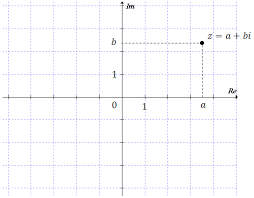
\includegraphics[width=\linewidth]{uz.png}
			\end{minipage}
	}
	
	\item Podać postać trygonometryczną liczby zespolonej; zdefiniować moduł liczby zespolonej.
	\Odp{
		$$z=a+ib$$
		$$z=r(\cos\varphi + i\sin\varphi)$$
		$$|z|=\sqrt{a^2+b^2}$$
	}
	\newpage
	\item Uzasadnić, dlaczego niewłaściwym jest zapis liczby i jako $\sqrt{-1}$.
	\Odp{
		$\sqrt{-1}$  jest to zbiór elementowy $\{i,-i\}$, a nie jedna liczba.
	}
	
	\item Podać „dowód” błędnego faktu, że $1 = -1$ z wykorzystaniem zapisu „$\sqrt{-1}$” i pokazać	błąd w tym dowodzie.
	\Odp{
		$$\sqrt{-1}=\sqrt{-1}$$
		$$\sqrt{\frac{-1}{1}}=\sqrt{\frac{1}{-1}}$$
		$$\frac{\sqrt{-1}}{\sqrt{1}}=\frac{\sqrt{1}}{\sqrt{-1}}$$
		$$\sqrt{-1}\cdot\sqrt{-1}=\sqrt{1}\cdot\sqrt{1}$$
		$$-1=1$$
	}
	
	\item Określić (ogólnie) historię znajdywania wzorów ogólnych na rozwiązywanie równań n-tego stopnia (co zrobili: Tartaglia, Cardano, Ferrari, Abel, Galois).
	\Odp{
		\textbf{Tartaglia} – w XVI wieku odkrył metodę rozwiązywania równań sześciennych w szczególnym przypadku (tzw. równania zredukowanego). Przekazał swój sposób Girolamo Cardano pod warunkiem zachowania go w tajemnicy.
		
		\textbf{Cardano} – opublikował w 1545 r. w \emph{Ars Magna} ogólny wzór na pierwiastki równań sześciennych, wykorzystując metodę Tartaglii i własne uogólnienia. Jego praca zapoczątkowała rozwój algebry symbolicznej.
		
		\textbf{Ferrari} – uczeń Cardana, rozwiązał ogólnie równania czwartego stopnia (równania bi-kwadratowe) – jego metoda opiera się na sprowadzeniu równania czwartego stopnia do dwóch równań kwadratowych.
		
		\textbf{Abel} – w 1824 roku udowodnił, że nie istnieje ogólny wzór (wyrażony przez pierwiastki) dla równań algebraicznych stopnia piątego i wyższego. To był przełom w rozumieniu granic klasycznej algebry.
		
		\textbf{Galois} – rozwinął teorię grup i stworzył podstawy teorii Galois, która pozwala precyzyjnie określić, kiedy dane równanie algebraiczne da się rozwiązać przez pierwiastki. Pokazał, że rozwiązanie zależy od struktury grupy permutacji pierwiastków równania.
	}
	
	
	\item Sformułować zasadnicze twierdzenie algebry.
	\Odp{
		Dowolny wielomian $n$-tego stopnia ma dokładnie $n$ pierwiastków zespolonych wraz z krotnościami.
	}
	\newpage
	\item Zdefiniować kwaterniony.
	\Odp{
		$\mathbb{R}^4 \qquad \begin{bmatrix}
			a+ib+jc+kd\\
			i^2=j^2=k^2=ijk=-1
		\end{bmatrix} \Rightarrow ij=k, ik=j, jk=i, ijk=-1, ijkk=-k, -ij=-k, ij=k$
	}
	
	\item Zdefiniować liczby naturalne na bazie zbiorów.
	\Odp{
		\begin{itemize}
			\item $\emptyset$ - 0 elementów
			\item $\{\emptyset\}$ - 1 element
			\item $\{\emptyset,\{\emptyset\}\}$ - 2 elementy
			\item $\{\emptyset,\{\emptyset\},\{\emptyset,\{\emptyset\}\}\}$ - 3 elementy
			\item $\{\emptyset,\{\emptyset\},\{\emptyset,\{\emptyset\}\},\{\emptyset,\{\emptyset\},\{\emptyset,\{\emptyset\}\}\}\}$ - 4 elementy
			\item itd.
		\end{itemize}
	}
	
	\item Zdefiniować liczby naturalne wg aksjomatów Peano.
	\Odp{
			$\mathbb{N}$, operacja następnika $a \rightarrow N(a)$
			\begin{enumerate}[1)]
				\item $1\in \mathbb{N} \qquad (0\in \mathbb{N})$
				\item $\forall_{a\in\mathbb{N}} N(a)\neq 1$
				\item $\forall_{a\in \mathbb{N}} a$ ma dokładnie jeden następnik
				\item $N(a)=N(b) \Leftrightarrow a=b$
				\item $\begin{bmatrix}
					A\subset \mathbb{N}\\
					1\in A\\
					n\in A \Rightarrow n+1\in A
				\end{bmatrix} \Rightarrow A=\mathbb{N}$
			\end{enumerate}
	}
	
	\item Zdefiniować liczby naturalne wg aksjomatów Wilkosza.
	\Odp{
	\begin{enumerate}[1)]
		\item $\exists_n : n\in\mathbb{N}$ ($\neq \emptyset$)
		\item $\forall_{k\in\mathbb{N}} \exists_{n\in\mathbb{N}}:k<n$ (nie ograniczony z góry)
		\item $\forall_{k,n\in \mathbb{N}} k<m \Rightarrow ~(m<k)$ (antysymetria)
		\item $(A\subset\mathbb{N}, \exists_{k\in A})(\neq\emptyset) \Rightarrow \exists_{i\in A} \forall_{n\in A} i\leq n$ (zasada minimum)
		\item $(A\subset\mathbb{N}, \exists_{k\in A})(\neq\emptyset)$ oraz  $ (\exists_{i\in \mathbb{N}} \forall_{m\in A} m\leq i)\Rightarrow \exists_{k\in A} \forall_{l\in A} l\leq j$ (ograczinony z góry ma element największy)
	\end{enumerate}
	}
	\newpage
	\item Sformułować zasadę indukcji matematycznej z użyciem zapisu „$T_n$” (własność prawdziwa dla liczby naturalnej $n$).
	\Odp{
		$A\subset \mathbb{N}$\\\\
		
		$\begin{bmatrix}
			1) & n_0\in A\\
			2) & \forall_{n\geq n_0} n\in A \Rightarrow n+a\in A
		\end{bmatrix} \Rightarrow A \supset \mathbb{N}_{n_0}$\\\\
		
		$T_n$ - własność dotycząca liczby naturalnej $n$ jest prawdziwe\\\\
		
		$\begin{bmatrix}
			1) & T_n\\
			2) & \forall_{n\geq n_0} T_n\Rightarrow T_{n+1}
		\end{bmatrix} \Rightarrow \forall_{n\geq n_0} T_n$
	}
	
	\item Sformułować zasadę indukcji matematycznej zapisaną za pomocą należenia liczb naturalnych do pewnego zbioru.
	\Odp{
		$A\subset N$
		
		$\begin{bmatrix}		
			1^\circ &n_0\in A\\
			2^\circ &\forall_{n\geq n_0} n\in A \Rightarrow n+1\in A
		\end{bmatrix}
		\Rightarrow A\supset \mathbb{N}_{n_0}$
	}
	
	\item Sformułować zasadę indukcji matematycznej z założeniem w drugim kroku dotyczącym „wszystkich poprzedzających liczb”.
	\Odp{
		Tak zwana \textbf{zasada indukcji zupełnej}
		
		$\begin{bmatrix}
			1) &0\in B\\
			2) &(indukcja) n\in B\Rightarrow 0,\dots,n \in B\\
		\end{bmatrix}\Rightarrow B=\mathbb{N}$
	}
	
	\item Sformułować zasadę indukcji matematycznej „z przeskokiem o dwie liczby”.
	\Odp{
		\begin{enumerate}[1)]
			\item $T_0,T_1$
			\item $\forall_n\geq 0 (T_n\Rightarrow T_n+2)$
		\end{enumerate}
	
		$\Rightarrow \forall_{n\in \mathbb{N}} T_n$
	}
	\newpage
	\item Sformułować zasadę indukcji matematycznej w wersji indukcji wstecznej.
	\Odp{
		$\begin{bmatrix}
			1)& T_0\\
			2)& \exists_{n_k}, n_k \rightarrow \infty (k\rightarrow \infty), n_0 = 0, (n_k)$ - silnie rosnący $T_{n_k} \Rightarrow T_{n_{k+1}}\\
			3)& \forall_n\geq 1 T_n \Rightarrow T_{n-1}
		\end{bmatrix} \Rightarrow \forall_{n\in\mathbb{N}} T_n$
	}
	
	\item Udowodnić równoważność zasady indukcji matematycznej z zasadą minimum.
	\Odp{
		Zasada minimum $\Leftrightarrow$ Zasada indukcji matematycznej
		
		"$\Rightarrow$"
		
		$\begin{bmatrix}
			0\in A\\
			\forall_{n\geq 0} n\in A \Rightarrow n+1\in A
		\end{bmatrix} \overset{?}{\Rightarrow} A=\mathbb{N} $
	
		Hp. $A\neq \mathbb{N}$
		
		$B:= \mathbb{N}\setminus A, B\neq \emptyset$
		
		$0\in A \Rightarrow 0\notin B$
		
		Niech $k_0:= min B, k_0 >0$
		
		$k_0-1 \in \mathbb{N}, k_0-1\in B, k_0-1\in A$
		
		$k_0-1+1 = k_0 \in A$ sprzeczność\\\\
		
		"$\Leftarrow$"
		
		$A\subset \mathbb{N}$, w $A$ nie ma elementu najmniejszego $\overset{?}{\Rightarrow} A=\emptyset$
		
		$0\notin A$, bo byłby najmniejszy
		
		$B:= \{ m\in \mathbb{N}:\forall_{k\leq m} k\notin A\}$
		
		\begin{enumerate}[I]
			\item $0\in B$
			\item (indukcja) $n\in B \Rightarrow 0,\dots,n\notin A$
			
			$n+1\notin A$ (bo gdyby $n+1\in A$ to $n+1$ byłby najmniejszy)
			
			$n+1\in B$
			
			$\overset{\text{indukcja}}{\Rightarrow} B=\mathbb{N}, \forall_{k\in \mathbb{N}} k\notin A \Rightarrow A=\emptyset$
		\end{enumerate}
	}
	\newpage
	\item Udowodnić indukcyjnie, że zbiór n-elementowy ma $2^n$ podzbiorów. Zwrócić szczególną uwagę na sformułowanie drugiego kroku indukcyjnego i odpowiednie podejście do jego dowodu.
	\Odp{
		\begin{enumerate}[$1^\circ$]
			\item $X=\emptyset$
			\item Z: $\forall_X \#X=n \Rightarrow \#P(X)=2^n$
				
				T: $\forall_Y : \#Y=n+1 \Rightarrow \#P(Y)=2^{n+1}$
				
				D: Niech $Y$ taki, że $\#Y=n+1$ oraz $a\in Y$
				
				$X:=Y\setminus \{a\}, \#X=n$
				
				Niech $B\subset Y,$ wtedy
				
				\begin{itemize}
					\item $a\in B \Rightarrow B=\{a\}\cup C$ - takich jest $2^n$
					
					lub\\
					
					\item $a\notin B \Rightarrow B\subset X$ - takich jest $2^n$
				\end{itemize}
			
			Czyli $2^n+2^n=2^{n+1}$.
		\end{enumerate}
	}
	
	\item Udowodnić nierówność między średnią arytmetyczną a geometryczną za pomocą indukcji wstecznej.
	\Odp{
		$a_1,\dots,a_n\geq 0 \Rightarrow \frac{a_1+\dots+a_n}{n}\geq \sqrt[n]{a_1\cdot \dots \cdot a_n}$
		
		\begin{enumerate}[I)]
			\item $n=1$
			
			$L=a_1$ $P=a_1$ ok
			
			\item $\forall_{n\geq 1} T_m\Rightarrow T_{2n}$
			
			Z:$x_1,\dots,x_n >0 \Rightarrow \sqrt[n]{x_1\cdot \dots \cdot x_n}\leq \frac{x_1+\dots+x_n}{n}$
			
			T:$y_1,\dots,y_{2n} >0 \Rightarrow \sqrt[2n]{y_1\cdot \dots \cdot y_{2n}}\leq \frac{y_1+\dots+y_{2n}}{2n}$
			
			D:$y_1,\dots,y_{2n}>0$
			
			$b_k:=\frac{y_{2k-1}+y_{2k}}{2}. c_k:=\sqrt{y_{2k-1}\cdot y_{2k}} \Rightarrow c_k\leq b_k$ (bo $a,b>0\Rightarrow \sqrt{ab}\leq \frac{a+b}{2}$)
			
			$\sqrt[2n]{y_1 \cdot \dots \cdot y_{2n}}=(y_1 \cdot \dots \cdot y_{2n})^\frac{1}{2n}=((y_1\cdot y_2)^\frac{1}{2}\cdot \dots \cdot (y_{2n-1}\cdot y_{2n})^\frac{1}{2})^\frac{1}{n}=(c_1\cdot \dots \cdot c_n)^\frac{1}{n}\underset{\text{z indukcji}}{\leq} \frac{c_1+\dots+c_n}{n}
			\leq \frac{b_1+\dots+b_n}{n}=\frac{y_1+\dots+y_{2n}}{2n}$
			
			\item $T_n\Rightarrow T_{n-1}, n\geq 2$
			
			Z: $x_1,\dots,x_n>0 \Rightarrow \sqrt[n]{x_1\dots x_n}\leq \frac{x_1+\dots+x_n}{2}$
			
			T:$a_1,\dots,z_{n-1}>0 \Rightarrow \sqrt[n-1]{a_1\dots a_{n-1}}\leq \frac{a_1+\dots+a_{n-1}}{n-1}$
				
			D:$a_1,\dots,a_{n-1}>0$
			
			$x_i=a_i$ $i=1,\dots,n-1$
			
			$x_n:=\sqrt[n-1]{a_1\dots a_{n-1}}=(a_1\dots a_{n-1})^\frac{1}{n-1}=(x_1\dots x_{n-1})^\frac{1}{n-1}\Rightarrow x_1\dots x_{n-1}=x_n^{n-1}$
			
			$\frac{x_1+\dots+x_n}{n}\geq (x_1\dots x_n)^\frac{1}{n}=(x_n^n)^{\frac{1}{n}}=x_n$
			
			$\frac{x_1+\dots+x_n}{n}+\frac{x_n}{n}\geq x_n$
			
			$\frac{x_1+\dots+x_{n-1}}{n}\geq x_n(1-\frac{1}{n})=x_n\frac{n-1}{n}$
			
			$\frac{x_1+\dots+x_{n-1}}{n-1}\geq x_n = \sqrt[n-1]{x_1\dots x_{n-1}}$
			
			$\frac{a_1+\dots+a_{n-1}}{n-1}\geq\sqrt[n-1]{a_1\dots a_{n-1}}$
			
			Indukcja wsteczna kończy dowód.
		\end{enumerate}
	}
	
	\item Udowodnić, że suma kątów w trójkącie wynosi $180^\circ$.
	\Odp{
		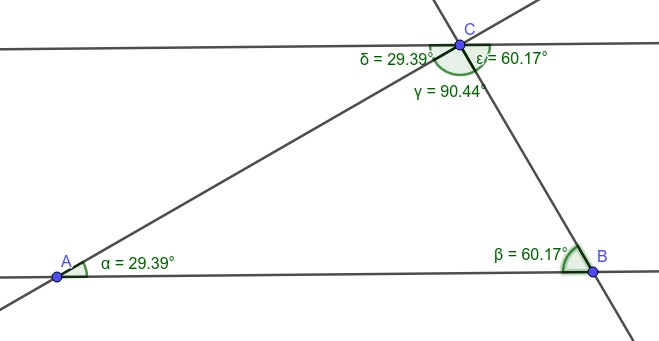
\includegraphics[width=0.7\linewidth]{tr180.jpeg}
		
		Kąty $\alpha$ i $\delta$ oraz $\beta$ i $\epsilon$ są odpowiednio sobie równe na podstawie katów naprzemianległych wewnętrznie.
		
		Suma kątów $\delta + \gamma + \epsilon$ jest kątem półpełnym, czyli ma $180^\circ$.
	}
	
	\item Udowodnić, że suma kątów w n-kącie wypukłym wynosi $(n - 2) \cdot 180^\circ$.
	\Odp{
		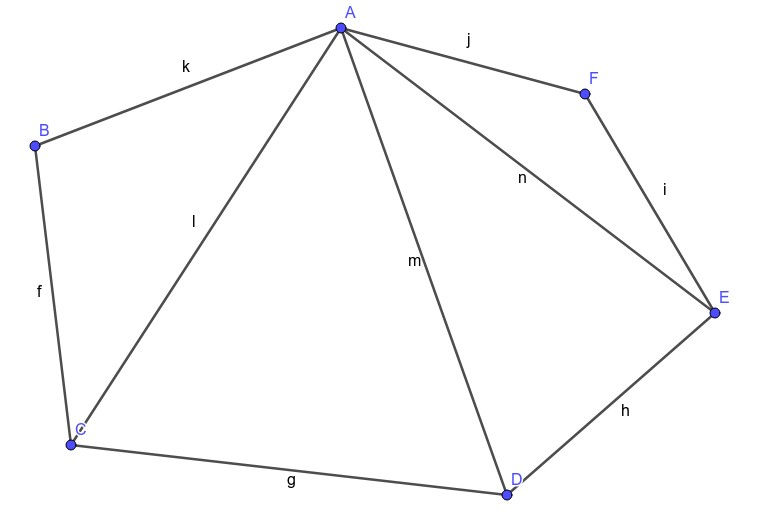
\includegraphics[width=0.7\linewidth]{wielo180.jpeg}
		
		Dowolny wielokąt wypukły o $n$ wierzchołkach można podzielić na $n-2$ trójkątów (w których kąty na siebie nie zachodzą), co daje nam w sumie $(n-2)\cdot 180^\circ$.
	}
	\newpage
	\item Udowodnić, że suma kątów w n-kącie wynosi $(n - 2) \cdot 180^\circ$, wykorzystując twierdzenie o istnieniu przekątnej zawartej w wielokącie.
	\Odp{
		\begin{enumerate}[I]
			\item ok
			\item W dolownym wielokącie istnieje przekątna zwarta w tym wielokącie.
			
			$T_3.\dots,T_n\Rightarrow T_{n+1}$
			
			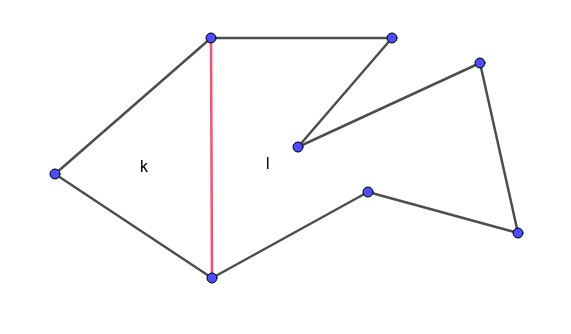
\includegraphics[width=\linewidth]{1ind180.jpeg}
			
			Przekątna dzieli $n+1$-kąt na $k$-kąt i $l$-kąt $(k,l\leq n, k+l=n+3)$.\\
			
			Suma kątów w $k$-kącie wynosi $(k-2)\cdot180^\circ$, podobnie w $l$-kącie wynosi $(l-2)\cdot180^\circ$.\\
			
			W $(n-1)$-kącie $(k-2)\cdot180^\circ + (l-2)\cdot180^\circ = (k+l-4)\cdot180^\circ=(n+3-4)\cdot180^\circ = (n-1)\cdot180^\circ =((n+1)-2)\cdot180^\circ$.\\
			
			Indukcja kończy dowód. 
		\end{enumerate}
	}
	\newpage
	\item Udowodnić, że suma kątów w n-kącie wynosi $(n - 2) \cdot 180^\circ$, wykorzystując twierdzenie o uchach (Two Ears Theorem).
	\Odp{
		\begin{enumerate}[I]
			\item ok
			\item W każdym wielokącie istnieją co najmniej 2 "ucha".
			
			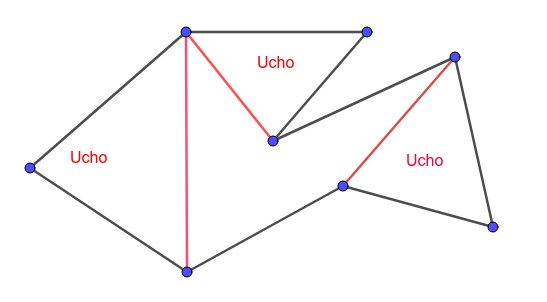
\includegraphics[width=\linewidth]{2ind180.jpeg}
			
			Bierzemy $(n+1)-kąt$. Ma in ucho $\Rightarrow$ odcinamy je. Powstaje $n$-kąt.
			
			$(n-2)\cdot180^\circ+180^\circ = (n-1)\cdot180^\circ = ((n+1)-2)\cdot180^\circ$
			
			Indukacja kończy dowód.
		\end{enumerate}
	}
	
	\item Pokazać, na czym polega błąd w indukcyjnym „dowodzie”, że suma kątów w n-kącie	wynosi $(n - 2) \cdot 180^\circ$, jeśli dowód przeprowadza się według schematu dodania trójkąta do n-kąta.
	\Odp{
		\textcolor{red}{TODO - Mam coś zapisane, ale brakuje mi dlaczego jest fałszywy - pewnie chodzi o "zepsucie" wypukłości wielokąta}
		
		\textbf{Od Przemka:} gdy dodamy trójkąt, to może się okazać, że otrzymamy wielokąt o tej samej liczbie wierzchołków co na początku - czyli nie ma właściwej realizacji kroku indukcyjnego
		
	}
	\newpage
	\item Podać błędny indukcyjny „dowód” tego, że wszystkie dziewczęta mają ten sam kolor oczu (lub wszystkie koty są tego samego koloru, itp.) i pokazać błąd w dowodzie.
	\Odp{
		Wszystkie dziewczęta mają ten sam kolor oczu.
		
		\begin{enumerate}[$1^\circ$]
			\item Jedna dziewczyna - ok
			\item Mam zbiór $n$ dziewczyn, dołączamy jedną dziewczynę tworząc zbiór $n+1$ elemetowy, następnie zabieramy dziewczynę z tej grupy (ale inną niż tą, która dołączaliśmy). Otrzymujemy zbiór $n$ elementowy, co z założeń indukcji daje nam, że wszystkie dziewnczyny mają ten sam kolor oczu. Czyli dołączona dziewczyna ma ten sam kolor oczu co pozostałe.
		\end{enumerate}
	
		Błąd polega na tym, że z $T_1\Rightarrow T_2$ mamy możliwą zamianę koloru oczu, ponieważ wymieniamy cały zbiór.
	}
	
	\item Uzasadnić, że „tricku” w „dowodzie” poprzedniej własności nie można stosować w „dowodzie” tego, że wszystkie koty są czarne. Pokazać błąd w „dowodzie” własności, że wszystkie koty są czarne.
	\Odp{
		To co wyżej.
	}
	
	\item Podać błędny indukcyjny „dowód” tego, że wszystkie liczby naturalne są równe i pokazać błąd w dowodzie.
	\Odp{
		$\forall_{m,n\in\mathbb{N}}: m=n$
		
		D (fałszywy): Chcemy pokazać, że $\forall_{k\in \mathbb{N}} \forall_{m,n\in\mathbb{N}} \max\{m,n\}=k \Rightarrow m=n$ 
			
			\begin{enumerate}[$1^\circ$]
				\item $k=0 \Rightarrow \max\{m,n\}=0 \Rightarrow m=n=0$ ok
				\item "$T_k\Rightarrow T_{k+1}$"
				
				$\max\{m,n\}=k+1$
				
				$\max\{m-1,n-1\}=k \overset{\text{zał ind}}{\Rightarrow} k=m-1=n-1 \Rightarrow m=n$
			\end{enumerate}
		Indukcja kończy dowód.
		
		Błąd polega na tym, że $m-1$ oraz $n-1$ nie muszą być naturalne.
	}
	
	\item Sformułować twierdzenie Pitagorasa.
	\Odp{
		W trójkącie prostokątnym suma kwadratów przyprostokątnych jest równa kwadratowi przeciwprostokątej.
		$$a^2+b^2=c^2$$
	}
	
	\item Sformułować i wykazać twierdzenie o odcinkach stycznych.
	\Odp{
		Niesłusznie zwane "najmocniejszym twierdzeniem algebry".
		
		Dany jest okrąg oraz punkt $P$ leżacy poza okręgiem. Z punktu $P$ poprowadzono dwie półproste styczne do okręgu odpowiednio w punktach $A$ i $B$. Wowczas:	$$|PA|=|PB|$$
		
	}
	\newpage
	\item Sformułować twierdzenie Talesa (z wszystkimi możliwymi proporcjami).
	\Odp{
		Dane są dwie proste nierównoległe oraz dwie proste równoległe przecinające te proste (zobacz rysunek).
		
		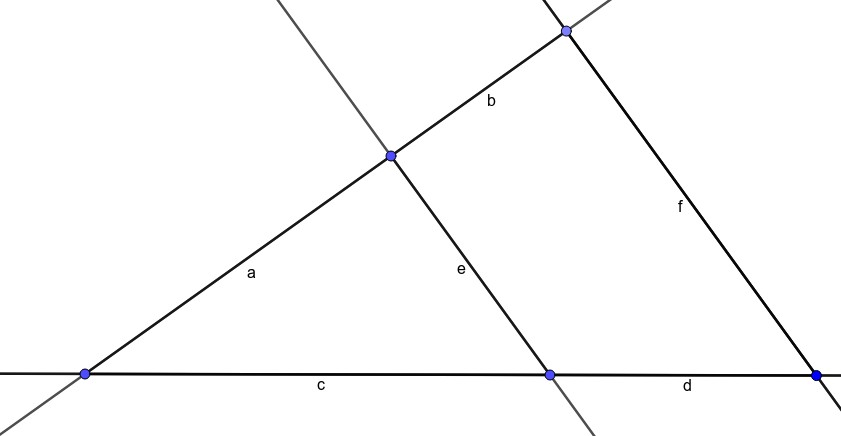
\includegraphics[width=0.7\linewidth]{tales.jpeg}
		
		Wówczas zachodzi:
		$$\frac{a}{c}=\frac{b}{d}=\frac{a+b}{c+d}\qquad\frac{a}{a+b}=\frac{c}{c+d}=\frac{e}{f}$$
	}
	
	\item Udowodnić twierdzenie Talesa metodą z „Elementów” Euklidesa.
	\Odp{
		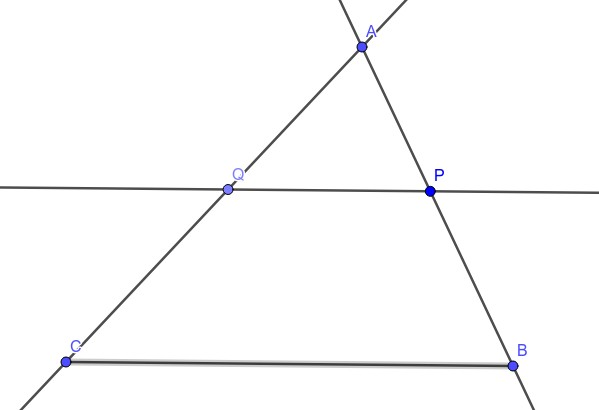
\includegraphics[width=0.7\linewidth]{tales_proof.jpeg}
		
		$$\frac{AP}{BP}=\frac{P_{\Delta APQ}}{P_{\Delta BPQ}}=\frac{P_{\Delta APQ}}{P_{\Delta QPC}}=\frac{AQ}{CQ}$$
	}
	\newpage
	\item Wykazać, że jeśli w trójkącie dwa boki są równe, to i dwa kąty są równe.
	\Odp{
		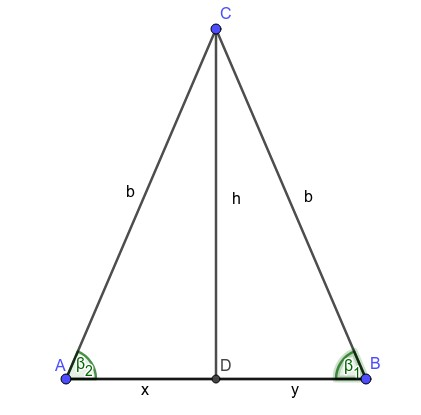
\includegraphics[width=0.5\linewidth]{trj_proof_1.jpeg}
		
		$x=\sqrt{b^2-h^2}=y \Rightarrow x=y \Rightarrow \beta_1=\beta_2$, bo tą przystające.
	}
	
	\item Wykazać, że jeśli w trójkącie dwa boki są równe, to i dwa kąty są równe bez wykorzystywania Aksjomatu V Euklidesa (czyli bez twierdzenia Pitagorasa).
	\Odp{
		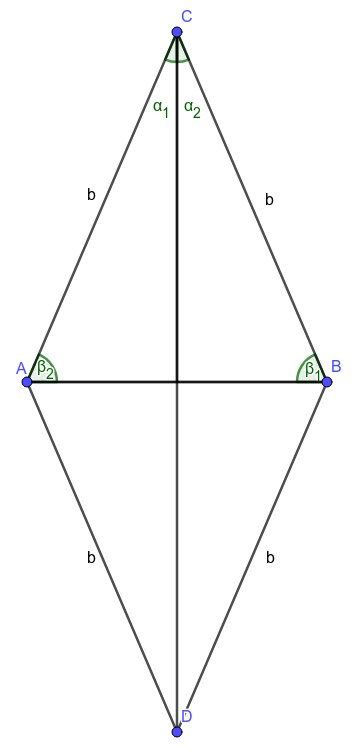
\includegraphics[width=0.3\linewidth]{trj_proof_2.jpeg}
		
		$\Delta ABD$ i $\Delta ABD$ przystajce (cecha BBB) $\Rightarrow \alpha_1=\alpha_2\Rightarrow$ trójkąty u góry są przystające $\Rightarrow \beta_1=\beta_2$
	}
	\newpage
	\item Wykazać, że jeśli w trójkącie dwa kąty są równe, to i dwa boki są równe.
	\Odp{
		$\alpha_1=\alpha_2\Rightarrow \Delta$ przystające $\Rightarrow b_1=b_2$
	}
	
	\item Wykazać, że jeśli w trójkącie dwa kąty są równe, to i dwa boki są równe bez wykorzystywania Aksjomatu V Euklidesa (czyli bez korzystania z tego, że suma kątów w trójkącie wynosi $180^\circ$).
	\Odp{
		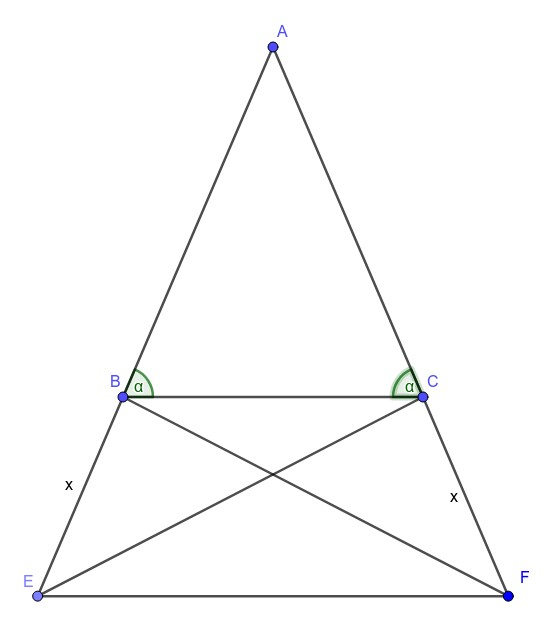
\includegraphics[width=0.4\linewidth]{trj_proof_4.jpeg}
		
		Trójkąty $ABF$ i $ACE$ są przystające (cecha BKB). $\Rightarrow$ $\angle AEC = \angle BFA \Rightarrow |CE| = |CF| \Rightarrow |AB|=|AC|$
	}
	
	\item Udowodnić, że symetralne boków trójkąta przecinają się w jednym punkcie.
	\Odp{
		Niech punkt $O$ oznacza przecięcie się dwóch symetralnych - boku AB i BC. Wówczas
		
		$
		\begin{bmatrix}
			\text{sym} AB \Rightarrow |AO|=|OB|\\
			\text{sym} BC \Rightarrow |OB|=|OC|
		\end{bmatrix} \Rightarrow |AO| = |OC| \Rightarrow O \in \text{sym} AC
		$.
		
	}
	\newpage
	\item Udowodnić, że wysokości w trójkącie (precyzyjnie: proste zawierające wysokości w trójkącie) przecinają się w jednym punkcie.
	\Odp{
		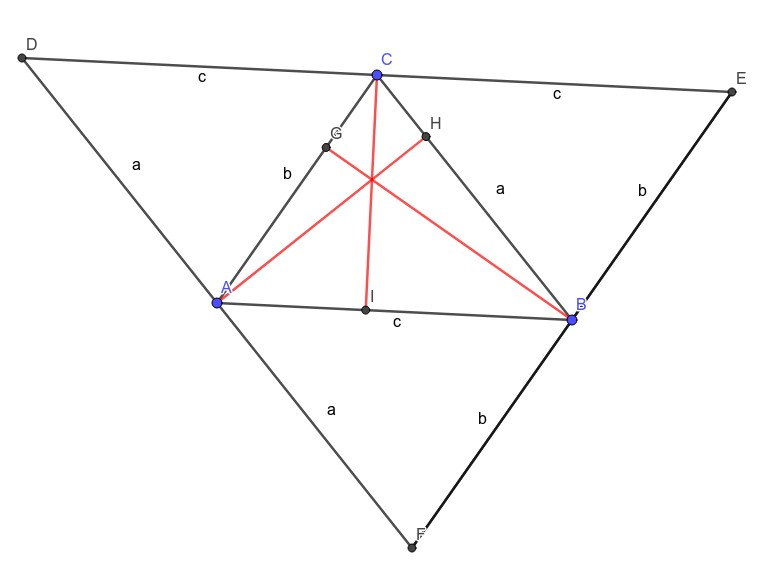
\includegraphics[width=0.6\linewidth]{trj_proof_6.jpeg}
		
		Tworzymy proste równoległe do podtaw jak rysunek wyżej. Czerwone linie zawierają się w symetrialych $\Rightarrow$ przecinają się w jednym punkcie.
	}
	
	\item Udowodnić, że dwusieczne kątów trójkąta przecinają się w jednym punkcie.
	\Odp{
		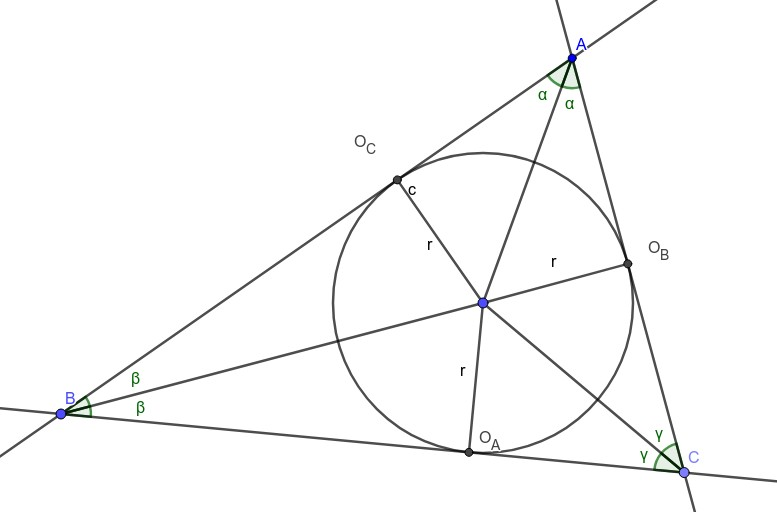
\includegraphics[width=0.6\linewidth]{trj_proof_7.jpeg}
		
		Dwusieczne kątów $\angle ABC$ i $\angle ACB$ musza się przecinać.
	
		Wówczas $OO_B=OO_A \wedge OO_C=OO_A \Rightarrow OO_C=OO_B$, czyli jest to dwusieczna kąta $\angle BAC$ 
	}
	\newpage
	\item Udowodnić, że środkowe w trójkącie przecinają się w jednym punkcie, dzielącym każdą	ze środkowych w stosunku $1:2$.
	\Odp{
		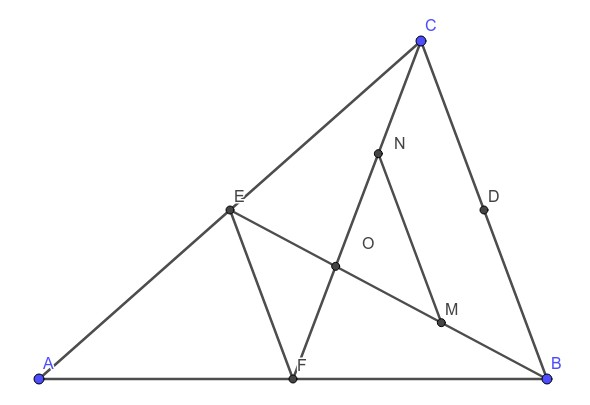
\includegraphics[width=0.6\linewidth]{trj_proof_8.jpeg}
		
		Dorysowuwuje odcinek $EF$ równoległy do $BC$ (odwrotne tw. Talesa)
		
		Dziele $AO$ i $CO$ w połowie (punkty $M$ i $N$) $(|MN|\: ||\: |EF|)$
		
		Z twierdzenia Talesa $\frac{FE}{BC}=\frac{MN}{BC}=\frac{1}{2} \Rightarrow MN=EF \Rightarrow MNEF$ jest równoległobokiem.
		
		$O$ - środek równoległoboku, przekątne przecinają się w połowie.
		
		Czyli $O$ dzieli $CF$, $BE$ w stosunku $1:2$ 
	}
	
	\item Zdefiniować funkcję, dziedzinę funkcji, przeciwdziedzinę funkcji.
	\Odp{
		$X,Y$ - zbiory, $X,Y\neq \emptyset$
		
		$f:X\rightarrow Y \Leftrightarrow \forall_{x\in X} \exists!_{y\in Y}: (x,y)\in f$
		
		$X$ - dziedzina
		
		$Y$ - przeciwdziedzina
	}
	
	\item Zdefiniować obraz i przeciwobraz (przy danej funkcji).
	\Odp{
		$f(A):= \{f(x):x\in A\}, A\subset X$ nazywamy obrazem zbioru A
		
		$f^{-1}(B):= \{x\in X: f(x)\in B\}, b\subset B$ nazywamy przeciwobrazem zbioru B 
	}
	
	\item Wyjaśnić różnicę między symbolami "$\longrightarrow$" i „$\longmapsto$”.
	\Odp{
		$\longrightarrow$ - służy do określenia relacji między zbiorami
		
		$\longmapsto$ - opiusje działanie funkcji na konkretnych elementach
		
		Np. $f:\mathbb{C} \longrightarrow \mathbb{R}, \qquad z\longmapsto \text{Re}z$
	}
	\newpage
	\item Zdefiniować injekcję, surjekcję i bijekcję.
	\Odp{
		Injekcja ($f$ różnowartościowa) $\Leftrightarrow f(x_1)=f(x_2)\Rightarrow x_1=x_2$ ($x_1\neq x_2 \Rightarrow f(x_1)\neq f(x_2)$)
		
		Surjekcja ($f$ - "na $Y$") $\Leftrightarrow \forall_{y\in Y} \exists_{x\in X} : f(x)=y$
		
		Bijekcja = Injekcja + Surjekcja
	}
	
	\item Podać różne metody określania funkcji.
	\Odp{
		\begin{itemize}
			\item przepis (w tym wzór)
			\item tableka
			\item graf
			\item wykres
		\end{itemize}
	}
	
	\item Wykazać, że funkcja dana wzorem: $f (k, n) = \frac{(n+k)(n+k+1)}{2}+k$ jest bijekcją z $\mathbb{N}^2$ na $\mathbb{N}$.
	\Odp{
		Czy surjekcja? $s\in \mathbb{N}$
		
		(?) $\exists_{k,n\in\mathbb{N}}: f(k,n)=s$
		
		$\exists_p: \frac{p(p+1)}{2}\leq s < \frac{(p+1)(p+2)}{2}$
		
		$k:=s-\frac{p(p+1)}{2}$ 
		
		$p=n+k\Rightarrow n=p-k = p-s+\frac{p(p+1)}{2}=\frac{2p+p(p+1)}{2}-s=\frac{p(p+3)}{2}-s$
		
		$n:=\frac{p(p+3)}{2}-s$
	
		$k+n=s-\frac{p(p+1)}{2}+\frac{p(p+3)}{2}-s=\frac{p(p+3-p-1)}{2}=\frac{2p}{p}=p$
		
		$f(k,n)=\frac{(k+n)(k+n+1)}{2}+k=\frac{p(p+1)}{2}+s-\frac{p(p-1)}{2}=s$\\\\
		
		Czy injekcja?	
		
		(?) $f(k,n) = f(\bar{k},\bar{n})\Rightarrow k=\bar{k}, n=\bar{n}$
		
		\begin{enumerate}[1$^\circ$]
			\item $k+n\neq \bar{k}+\bar{n} \qquad$ np. $k+n<\bar{k}+\bar{n} \Rightarrow k+n+1\leq \bar{k}+\bar{n}$\\
			
			$f(k,n)=\frac{{(n+k)(n+k+1)}{2}+k}{2}< \frac{{(n+k)(n+k+1)}{2}+k+n+1}{2} = \frac{(k+n)(k+n+1)+2(k+n+1)}{2}=$ 
			
			$=\frac{(k+n+1)(k+n+2)}{2}\leq \frac{(\bar{k}+\bar{n})(\bar{k}+\bar{n}+1)}{2}\leq f(\bar{k},\bar{n})$
			
			\item $k+n=\bar{k}+\bar{n}$
			
			$f(k,n)=f(\bar{k}m\bar{n})$
			
			$\frac{(k+n)(k+n+1)}{2}+k=\frac{(\bar{k}+\bar{n})(\bar{k}+\bar{n}+1)}{2}+\bar{k}=\frac{(k+n)(k+n+1)}{2}+\bar{k}$
			
			$k=\bar{k} \Rightarrow n=\bar{n}$
		\end{enumerate}
	}
	\newpage
	\item Zdefiniować funkcję parzystą i funkcję nieparzystą.
	\Odp{
		$\emptyset\neq D \subset \mathbb{R}$, $D$ symetryczny względem $0$ $(x\in D\Leftrightarrow -x\in D)$
		
		$f:D\rightarrow\mathbb{R}$ - parzysta $\Leftrightarrow \forall_{x\in D} f(x)=f(-x)$
		
		$f:D\rightarrow\mathbb{R}$ - nieparzysta $\Leftrightarrow \forall_{x\in D} f(x)=-f(-x) \qquad (f(-x)=-f(x))$
	}
	
	\item Wykazać, że jeśli dziedzina funkcji rzeczywistej jest zbiorem symetrycznym względem 0, to funkcja ta jest sumą funkcji parzystej i funkcji nieparzystej.
	\Odp{
		$f:D\rightarrow \mathbb{R}$, $D$ symetryczny względem $0$
		
		T: $\exists g,h : D\rightarrow \mathbb{R}$, $g$ - parzysta. $h$ - nieparzysta $: f=g+h$
		
		D: Zdefiniujmy $g(x):=\frac{f(x)-f(-x)}{2}$, $h(x):=\frac{f(x)+f(-x)}{2}$. Wówczas
		\begin{itemize}
			\item $g(x)=g(-x)$
			\item $h(-x)=\frac{f(-x)-f(x)}{2}=\frac{-f(x)-f(-x)}{2}=-h(x)$
		\end{itemize}
		
		$g(x)+h(x)=\frac{f(x)-f(-x)+f(x)+f(-x)}{2}=\frac{2f(x)}{2}=f(x)$  
	}
	
	\item Zdefiniować funkcję rosnącą, funkcję malejącą, funkcję silnie rosnącą, funkcję silnie malejącą.
	\Odp{
		$$f-\text{ rosnąca } \Leftrightarrow \forall_{x_1,x_2\in D}\; x_1<x_2\Rightarrow f(x_1)\leq f(x_2)$$
		$$f-\text{ malejąca } \Leftrightarrow \forall_{x_1,x_2\in D}\; x_1<x_2\Rightarrow f(x_1)\geq f(x_2)$$
		$$f-\text{ silnie rosnąca } \Leftrightarrow \forall_{x_1,x_2\in D}\; x_1<x_2\Rightarrow f(x_1)< f(x_2)$$
		$$f-\text{ silnie malejąca } \Leftrightarrow \forall_{x_1,x_2\in D}\; x_1<x_2\Rightarrow f(x_1)> f(x_2)$$
		
	}
	
	\item Podać i udowodnić twierdzenie o złożeniu funkcji rosnących, o złożeniu funkcji malejących, o złożeniu funkcji rosnącej z funkcją malejącą, o złożeniu funkcji malejącej z funkcją rosnącą.
	\Odp{
		Niech $f,g$ - rosnące, wówczas $g\circ f$ jest funkcją rosnącą.
		
		D: $x_1<x_2 \Rightarrow f(x_1)\leq f(x_2) \Rightarrow g(f(x_1))\leq g(f(x_2))$\\\\
		
		Niech $f$ - rosnąca, $g$ - malejąca, wówczas $g\circ f$ jest funkcją malejącą.
		
		D: $x_1<x_2 \Rightarrow f(x_1)\leq f(x_2) \Rightarrow g(f(x_1))\geq g(f(x_2))$\\\\
		
		Niech $f,g$ - malejące, wówczas $g\circ f$ jest funkcją rosnącą.
		
		D: $x_1<x_2 \Rightarrow f(x_1)\geq f(x_2) \Rightarrow g(f(x_1))\leq g(f(x_2))$
	}
	
	\item Wykazać, że jeśli złożenie dwóch funkcji jest bijekcją, to funkcja wewnętrzna jest	injekcją, a funkcja zewnętrzna surjekcją.
	\Odp{
		D: 
		\begin{enumerate}[(1)]
			\item Hp. $\exists_{x_1,x_2} x_1\neq x_2 f(x_1)=f(x_2)$
			
			$g(f(x_1))=g(f(x_2))$
			
			$(g\circ f)(x_1)=(g\circ f)(x_2)$ sprzeczność
			
			\item $z\in Z \exists_{x\in X} (g\circ f)(x)=z$
			
			$g(f(x))=z$
			
			$y=f(x)\in Y$, $g(f(x))=z$ ok 
		\end{enumerate}
	}
	
	\item Zdefiniować funkcję okresową w przypadku, gdy dziedzina tej funkcji jest podzbiorem	$\mathbb{R}$.
	\Odp{
		Niech $f:D\rightarrow \mathbb{R}$, wtedy
		
		$f-\text{ okresowa } \Leftrightarrow \exists_{T>0}: \forall_{x\in D} : x+T\in D, \underline{x-T\in D} \Rightarrow  f(x)=f(x+T)\underline{=f(x-T)}$\\\\
		
		\underline{Ta część} jest niepotrzebna, bo $f(x-T+T)=f(x)$
	}
	
	\item Zdefiniować funkcję okresową w przypadku, gdy dziedzina tej funkcji jest równa $\mathbb{R}$.
	\Odp{
		Niech $f:\mathbb{R}\rightarrow \mathbb{R}$, wtedy
		
		$f-\text{ okresowa } \Leftrightarrow \exists_{T>0}: \forall_{x\in \mathbb{R}} f(x)=f(x+T)$
		
	}
	
	\item Zdefiniować funkcję Dirichleta i podać jej okresy.
	\Odp{
		$$\chi_{\mathbb{Q}}(x)=\UkladRownan{1 \text{ gdy } x\in\mathbb{Q}}{0 \text{ gdy } x\notin\mathbb{Q}}$$
		Okresem tej funkcji jest każde $p\in\mathbb{Q}: p>0$.
	}
	\newpage
	\item Podać przykład funkcji niestałej, której okresami są 1 oraz $\sqrt{2}$.
	\Odp{
		$$g(x)=\UkladRownan{1 \text{ gdy } x=a+b\sqrt{2}: a,b\in \mathbb{Z}}{0 \text{ dla pozostałych } x}$$
		
		D: Niech $x$ ma postać $a+b\sqrt{2}$, wówczas:
		$$x+1=(a+1)+b\sqrt{2}$$
		
		$$x+\sqrt{2}=a+(b+1)\sqrt{2}$$
		
		Niech $x$ nie ma postaci $a+b\sqrt{2}$
		
		Hp. $x+1=c+d\sqrt{2} \Rightarrow x=(c-1)+d\sqrt{2}$ sprzeczność
		
		Hp. $x+\sqrt{2}=c+d\sqrt{2} \Rightarrow x= c+(b-1)\sqrt{2}$ sprzeczność
	}
	
	\item Zdefiniować funkcje sinus, cosinus, tangens, cotangens dla kąta ostrego.
	\Odp{
		$$\sin\alpha=\frac{\text{długość przyprostokątnej przeciwległej do danego kąta } \alpha}{\text{długość przeciwprostokątnej tego trójkąta}}$$
		$$\cos\alpha=\frac{\text{długość przyprostokątnej przyległej do danego kąta } \alpha}{\text{długość przeciwprostokątnej tego trójkąta}}$$
		$$\tg\alpha=\frac{\text{długość przyprostokątnej przeciwległej do danego kąta } \alpha}{\text{długość przyprostokątnej przyległej do danego kąta } \alpha}$$
		$$\ctg\alpha=\frac{\text{długość przyprostokątnej przyległej do danego kąta } \alpha}{\text{długość przyprostokątnej przeciwległej do danego kąta } \alpha}$$
	}
	
	\item Uzasadnić, że powyższe definicje funkcji trygonometrycznych są postawione poprawnie.
	\Odp{
		Zostały dobrze zdefiniowane na podstawie podobieństwa trójkątów.
	}
	\newpage
	\item Zdefiniować funkcje sinus, cosinus, tangens, cotangens dla dowolnego kąta.
	\Odp{
		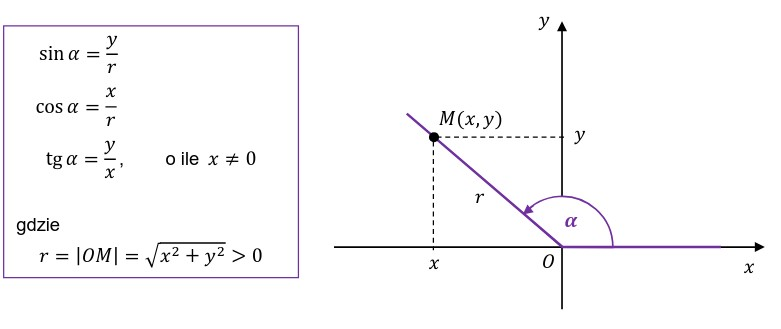
\includegraphics[width=\linewidth]{tryg_def.jpeg}
	}
	
	\item Uzasadnić, że powyższe definicje funkcji trygonometrycznych są postawione poprawnie.
	\Odp{
		Są zdefiniowane poprawnie z podobieństwa trójkątów. Co więcej są uogólnieniem poprzedniej definicji funkcji trygonometrycznych na trójkącie protokątnym.
	}
	
	\item Uzasadnić, że definicje funkcji trygonometrycznych dla dowolnego kąta są uogólnieniem analogicznych definicji dla kąta ostrego.
	\Odp{
		Rozważając kat $\alpha$ ostry, otrzymujemy zwykły trójkąt prostokątny (gdzie sieczna jest przyprostokątną przeciwległą, rzędna jest przyprostokątną przyległa, a promień jest przeciwprostokątną).
	}
	
	\item Zdefiniować funkcje sinus, cosinus, tangens, cotangens dla argumentu zespolonego.
	\Odp{
		$\mathbb{C}$
		
		$\sin z=\sum_{n=0}^{\infty}(-1)^n\frac{z^{n+1}}{(2n+1)!}$
		
		$\cos z=\sum_{n=0}^{\infty}(-1)^n\frac{z^{2n}}{(2n)!}$
		
		$\tg z=\frac{\sin z}{\cos z} \qquad \ctg z=\frac{\cos z}{\sin z}$
	}
	
	\item Podać twierdzenie sinusów.
	\Odp{
		W dowolnym trójkącie zachodzi:
		$$\frac{a}{\sin\alpha}=\frac{b}{\sin\beta}=\frac{c}{\sin\gamma}=2R$$
	}
	\newpage
	\item Podać twierdzenie cosinusów.
	\Odp{
		W dowolnym trójkącie zachodzi:
		$$c^2=a^2+b^2-2ab\cos\gamma$$
		$$b^2=a^2+c^2-2ac\cos\beta$$
		$$a^2=b^2+c^2-2bc\cos\alpha$$
	}
	
	\item Wyrazić liczby $e^{iz}$ oraz $e^{-iz}$ za pomocą $\sin z$ oraz $\cos z$, udowodnić te wzory, znając w	szczególności wzór na $e^z$ za pomocą szeregu.
	\Odp{
		$$e^z=\sum_{n=0}^{\infty} \frac{z^n}{n!}$$\\\\
		
		$$e^{iz}=\sum_{n=1}^{\infty} i^n\frac{z^n}{n!}=
		\sum_{k=0}^{\infty}i^{2k}\frac{z^{2k}}{(2k)!}+\sum_{k=0}^{\infty}i^{2k+1}\frac{z^{2k+1}}{(2k+1)!}=$$
		
		 $$
		\sum_{k=0}^{\infty}(-1)^{k}\frac{z^{2k}}{(2k)!}+i\sum_{k=0}^{\infty}(-1)^{k}\frac{z^{2k+1}}{(2k+1)!}=\cos z + i\sin z$$\\\\
		
		$$e^{-iz}=\sum_{n=1}^{\infty} (-i)^n\frac{z^n}{n!}=
		\sum_{k=0}^{\infty}(-1)^{2k}(i)^{2k}\frac{z^{2k}}{(2k)!}+\sum_{k=0}^{\infty}(-1)^{2k+1}(i)^{2k+1}\frac{z^{2k+1}}{(2k+1)!}=$$
		
		$$\sum_{k=0}^{\infty}(-1)^{k}\frac{z^{2k}}{(2k)!}-i\sum_{k=0}^{\infty}(-1)^{k}\frac{z^{2k+1}}{(2k+1)!}=\cos z - i\sin z$$
		
	}
	
	\item Udowodnić wzór: $\sin^2 z + \cos^2 z = 1$ dla dowolnego kąta.
	\Odp{
		W dowolnym trójkącie prostokątnym zachodzi
		$$\sin^2\alpha+\cos^2\alpha=\frac{a^2}{c^2}+\frac{b^2}{c^2}=\frac{a^2+b^2}{c^2}=\frac{c^2}{c^2}=1$$	
	}
	\newpage
	\item Udowodnić wzór: $\sin^2 z + \cos^2 z = 1$ dla argumentu zespolonego.
	\Odp{
		$$\sin^2z+\cos^2z = (\cos z+i\sin z)(\cos z-i\sin z)=e^{iz}e^{-iz}=e^0=1$$
	}
	
	\item Podać wzory na sinus, cosinus i tangens sumy oraz różnicy kątów.
	\Odp{
		$$\sin(\alpha\pm\beta)=\sin\alpha\cos\beta\pm\cos\alpha\sin\beta$$
		$$\cos(\alpha\pm\beta)=\cos\alpha\cos\beta\mp\sin\alpha\sin\beta$$
		$$\tg(\alpha\pm\beta)=\frac{\tg\alpha\pm\tg\beta}{1\mp\tg\alpha\tg\beta}$$
	}
	
	\item Podać wzory na sumę i różnicę sinusów kąta, sumę i różnicę cosinusów kąta.
	\Odp{
		$$\sin\alpha+\sin\beta=2\sin\frac{\alpha+\beta}{2}\cos\frac{\alpha-\beta}{2}$$
		$$\sin\alpha-\sin\beta=2\cos\frac{\alpha+\beta}{2}\sin\frac{\alpha-\beta}{2}$$
		$$\cos\alpha+\cos\beta=2\cos\frac{\alpha+\beta}{2}\sin\frac{\alpha-\beta}{2}$$
		$$\cos\alpha-\cos\beta=-2\sin\frac{\alpha+\beta}{2}\cos\frac{\alpha-\beta}{2}$$
	}
	
	\item Podać mechanizm tworzenia wzorów redukcyjnych i stosować go w praktyce.
	\Odp{
		Sin, Cos i Tg poszły pić do baru.
		
		Na początku imprezy (I ćwiartka) wszystkie są w świetnym humorze – każda pije (Sin, Cos, Tg są dodatnie).
		
		W II ćwiartce Sin, która po angielsku znaczy "grzech", dalej pije, ale reszta już nie daje rady (Sin +, Cos i Tg -).
		
		W III ćwiartce Sin odpada z imprezy – wypiła za dużo (Sin -), Cos też nie pije, bo ma coś ważnego do zrobienia (Cos -), ale Tg jest „tenteges” i dalej pije (Tg +).
		
		W IV ćwiartce Cos wraca do siebie i coś tam jeszcze sączy (Cos +), ale Tg, która już piła dwa razy, odpuszcza (Tg -), a Sin wciąż nieprzytomna (Sin -).
		
		Tak oto wszystkie trzy maturzystki kończą imprezę – każda z innym bilansem.
	}
	\newpage
	\item Zdefiniować funkcje cyklometryczne: arc sin, arc cos, arc tg.
	\Odp{
		$\arcsin: [-1,1] \rightarrow [-\frac{\pi}{2},\frac{\pi}{2}]$
		
		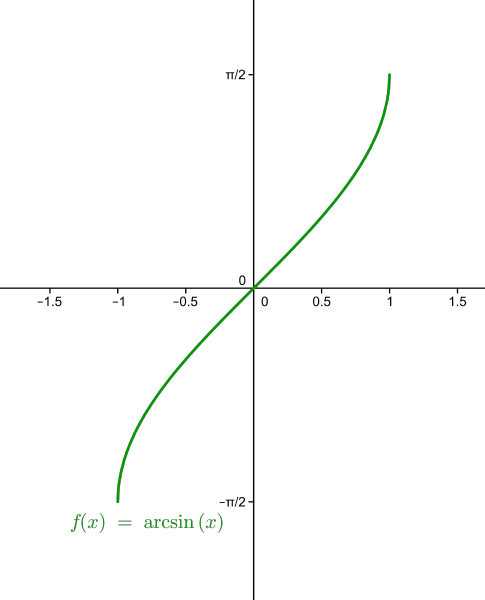
\includegraphics[width=0.4\linewidth]{arcsin.png}
		
		$\arccos: [-1,1] \rightarrow [0,\pi]$\\
		
		$\arctg: \mathbb{R} \rightarrow [-\frac{\pi}{2},\frac{\pi}{2}]$\\
		
		$\arcctg: \mathbb{R} \rightarrow [0,\pi]$
		
		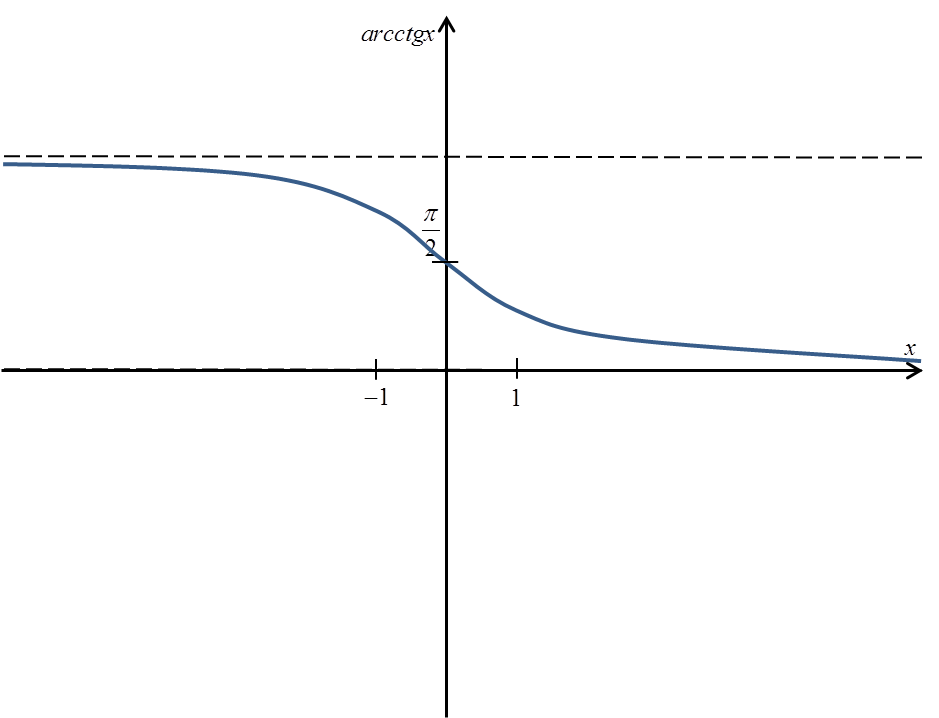
\includegraphics[width=0.4\linewidth]{arcctg.png}
	}
	
	\item Udowodnić, że $\sin 1^\circ$ jest liczbą niewymierną.
	\Odp{
		D: Hp. $\sin 1^\circ \in \mathbb{Q}$
		
		$\sin^2 1^\circ \in \mathbb{Q}$
		
		$\cos^21^\circ = 1- \sin^2 1^\circ \in \mathbb{Q}$
		
		$\cos 2^\circ = \cos^21^\circ - \sin^21^\circ \in \mathbb{Q}$
		
		$\sin^22^\circ = 1-\cos^22^\circ \in \mathbb{Q}$
		
		$\cos 4^\circ = \cos^22^\circ - \sin^22^\circ \in \mathbb{Q}$
		
		$\sin^24^\circ = 1-\cos^24^\circ \in \mathbb{Q}$
		
		$\cos 8^\circ = \cos^24^\circ - \sin^24^\circ \in \mathbb{Q}$
		
		$\sin^28^\circ = 1-\cos^28^\circ \in \mathbb{Q}$
		
		$\cos 16^\circ = \cos^28^\circ - \sin^28^\circ \in \mathbb{Q}$
		
		$\sin^216^\circ = 1-\cos^216\circ \in \mathbb{Q}$
		
		$\cos 32^\circ = \cos^216^\circ - \sin^216^\circ \in \mathbb{Q}$
		
		$\sin32^\circ= 2\sin16^\circ\cos16^\circ=4\sin8^\circ\cos8^\circ\cos16^\circ=8\sin4^\circ\cos4^\circ\cos8^\circ\cos16^\circ=$
		
		$=16\sin2^\circ\cos^\circ\cos4^\circ\cos8^\circ\cos16^\circ$
		
		$\mathbb{Q}\not\ni\frac{\sqrt{3}}{2} = \cos30^\circ = \cos(32^\circ - 2^\circ) = \cos32^\circ\cos2^\circ + \sin32^\circ\sin2^\circ=$
		
		$= \underset{\in \mathbb{Q}}{\cos32^\circ}\underset{\in \mathbb{Q}}{\cos2^\circ} + 16\underset{\in \mathbb{Q}}{\cos2^\circ}\underset{\in \mathbb{Q}}{\cos4^\circ}\underset{\in \mathbb{Q}}{\cos8^\circ}\underset{\in \mathbb{Q}}{\cos16^\circ}\underset{\in \mathbb{Q}}{\sin^22^\circ} \in \mathbb{Q}$ sprzeczność
	}
	
	\item Podać dwie równoważne definicje liczby pierwszej i wykazać ich równoważność.
	\Odp{
		Niech $p\in \mathbb{N}_+$.
		
		Def. 1 Liczba $p\in \mathbb{P}$ jeśli ma dokładnie dwa dzielniki\\
		$\Updownarrow$\\
		Def. 2 Liczba $p\in \mathbb{P}$ jeśli jest podzielna tylko przez 1 i samą siebie.\\\\
		
		D: "$\Rightarrow$"\\
		$p|p$, $1|p$, $p\neq1$ ok
		
		"$\Leftarrow$"
		$1|p$, $p|p$, $p\neq1$ $\Rightarrow$ ma dokładnie dwa dzielniki ok
		
	}
	
	\item Podać powód, dla którego jedynka nie jest uznawana za liczbę pierwszą.
	\Odp{
		Rozkład na czynniki pierwsze powinien być jednoznaczny, gdyby $1\in\mathbb{P}$, to np.
		
		$21=3^1\cdot7^1=1^\textbf{0}\cdot2^0\cdot3^1\cdot5^1\cdot7^0\cdot\dots=1^\textbf{6}\cdot2^0\cdot3^1\cdot5^1\cdot7^0\cdot\dots$
	}
	
	\item Udowodnić, że jeśli $p$ dzieli $a$ oraz $p$ dzieli $b$, to $p$ dzieli $a - b$
	\Odp{
		$p|a$ i $p|b$ $\Rightarrow p|(a-b)$
		
		D: $\exists_k:a=k\cdotp$ i $\exists_m:b=m\cdotp$ $\Rightarrow a-b=p(k-m) \Rightarrow p|p(k-m) \Rightarrow p|a-b$
	}
	
	\item Udowodnić, że liczb pierwszych jest nieskończenie wiele metodą Euklidesa.
	\Odp{
		Hp. Liczb pierwszych jest skończenie wiele $\mathbb{P}=\{p_1,p_2,\dots,p_n\}$.
		
		Weźmy liczbę $p:=p_1\cdotp_2\cdot\dots p_n + 1$. Wtedy $\forall_{p_i} p_i\not| p \Rightarrow p$ jest liczbą pierwszą. Sprzeczność. 
	}
	\newpage
	\item Udowodnić, że liczb pierwszych jest nieskończenie wiele metodą Kummera.
	\Odp{
		Hp. $p_1<p_2<\dots<p_n$ wszystkie liczby pierwsze.
		
		$p:=p_1\cdot p_2\cdot\dots\cdot p_n > 2$. Zalóżmy, że $p-1$ to iloczyn liczb pierwszych. Wówczas $\exists_j : p_j|p$ i $p_j|p-1$ $p_j|p-(p-1) \Rightarrow p_j|1$ sprzeczność
	}
	
	\item Udowodnić, że liczb pierwszych jest nieskończenie wiele metodą Stieltjesa.
	\Odp{
		Hp. Liczb pierwszych jest skończenie wiele $\mathbb{P}=\{p_1,p_2,\dots,p_n\}$.
		
		$p:=p_1\cdot p_2\cdot\dots\cdot p_n$
		
		$p=k\cdot m: k,m>1$
		
		$\forall_i p_i$ dzieli dokładnie jedną z liczb $k$ lub $m$
		
		Rozważmy $k+m>1$. Gdyby $\exists_{p_i}\:: p_i|k+m$, to
		
		$p_i|k \wedge p_i|k+m \Rightarrow p_i|k+m-k \Rightarrow p_i|m$ sprzeczność
		
		$p_i|m \wedge p_i|k+m \Rightarrow p_i|k+m-m \Rightarrow p_i|k$ sprzeczność
		
		Zatem $\forall_i \; p_i\not|k+m$, czyli $k+m$ to liczba pierwsza. Sprzeczność z hipotezą.
	}
	
	\item Udowodnić, że liczb pierwszych jest nieskończenie wiele metodą Eulera.
	\Odp{
		\begin{enumerate}[1)]
			\item $p\in\mathbb{P} \Rightarrow \frac{1}{p} \qquad \sum_{k=0}^{\infty}$
			\item $p,q$ - różne liczby pierwsze
			
			$(\sum_{k=0}^{\infty}\frac{1}{p^k})(\sum_{k=0}^{\infty}\frac{1}{q^k}) = \frac{1}{1-\frac{1}{p}}\cdot\frac{1}{1-\frac{1}{q}}=\sum \frac{1}{p^\alpha q^\beta} : \alpha,\beta\geq 0$ każda para $(\alpha,\beta)$ występuje dokładnie raz.
		\end{enumerate}
		
		Hp. $p_1,\dots,p_n$ różne liczby pierwsze
		
		$A=(\sum_{k=0}^{\infty}\frac{1}{p_1^k})\cdot(\sum_{k=0}^{\infty}\frac{1}{p_2^k})\cdot\dots\cdot(\sum_{k=0}^{\infty}\frac{1}{p_n^k})=\frac{1}{1-\frac{1}{p_1}}\cdot\frac{1}{1-\frac{1}{p_2}}\cdot\dots\cdot\frac{1}{1-\frac{1}{p_n}}\in(0,\infty)$
		
		Ale $A=\sum_{n=1}^{\infty}\frac{1}{n}=\infty$
		
		$n=p_1^{\alpha_1}\cdot \dots \cdot p_n^{\alpha_1}$ sprzeczność
	}
	\newpage
	\item Udowodnić, że dla każdej liczby naturalnej n większej od 2 w przedziale $[n, n!)$ znajduje
	się liczba pierwsza.
	\Odp{
		Tw. $\forall_{n\geq 2} \exists_{p\in\mathbb{P}} : p\in [n,n!)$
		
		D: Rozważmy liczbę $n!-1$
		\begin{enumerate}[$1^\circ$]
			\item $n!-1$ - liczba pierwsza $\Rightarrow$ ok
			\item $n!-1$ - liczba złożona $\Rightarrow$ $\exists_{p\in\mathbb{P}} : p|(n!-1) $
			
			Jeśli $p\leq n$ to $p|n! \Rightarrow p|n!-(n!-1) \Rightarrow p|1$ sprzeczność
			
			Zatem $p>n$
		\end{enumerate}
	}
	
	\item Podać zasadę tworzenia sita Eratostenesa.
	\Odp{
		\centering\begin{tabular}{|c|c|c|c|c|c|c|c|c|c|}\hline
			\sout{0}&\sout{1}&2&3&4&5&6&7&8&9\\\hline
			10&11&12&13&14&15&16&17&18&19\\\hline
			20&21&22&23&24&25&26&27&28&29\\\hline
		\end{tabular}
		$$\Downarrow$$
		\centering\begin{tabular}{|c|c|c|c|c|c|c|c|c|c|}\hline
			\sout{0}&\sout{1}&\textbf{2}&3&\sout{4}&5&\sout{6}&7&\sout{8}&9\\\hline
			\sout{10}&11&\sout{12}&13&\sout{14}&15&\sout{16}&17&\sout{18}&19\\\hline
			\sout{20}&21&\sout{22}&23&\sout{24}&25&\sout{26}&27&\sout{28}&29\\\hline
		\end{tabular}
		$$\Downarrow$$
		\centering\begin{tabular}{|c|c|c|c|c|c|c|c|c|c|}\hline
			\sout{0}&\sout{1}&\textbf{2}&\textbf{3}&\sout{4}&5&\sout{6}&7&\sout{8}&\sout{9}\\\hline
			\sout{10}&11&\sout{12}&13&\sout{14}&\sout{15}&\sout{16}&17&\sout{18}&19\\\hline
			\sout{20}&\sout{21}&\sout{22}&23&\sout{24}&25&\sout{26}&27&\sout{28}&29\\\hline
		\end{tabular}
		$$\Downarrow$$
		\centering\begin{tabular}{|c|c|c|c|c|c|c|c|c|c|}\hline
			\sout{0}&\sout{1}&\textbf{2}&\textbf{3}&\sout{4}&\textbf{5}&\sout{6}&\textbf{7}&\sout{8}&\sout{9}\\\hline
			\sout{10}&\textbf{11}&\sout{12}&\textbf{13}&\sout{14}&\sout{15}&\sout{16}&\textbf{17}&\sout{18}&\textbf{19}\\\hline
			\sout{20}&\sout{21}&\sout{22}&\textbf{23}&\sout{24}&\sout{25}&\sout{26}&\sout{27}&\sout{28}&\textbf{29}\\\hline
		\end{tabular}
	}
	
	\item Sformułować twierdzenie Greena-Tao.
	\Odp{
		$\forall_n$ istnieje ciąg arytmetyczny złożony z $n$ liczb pierwszych.
	}
	
	\item Wykazać, że nie istnieje nieskończony ciąg arytmetyczny, którego wyrazami są jedynie
	liczby pierwsze.
	\Odp{
		D: Niech $p$ - pierwszy wyraz tego ciągu (liczba pierwsza)
		
		Hp. $\exists_r : r$ - różnica tego ciągu i wszystkie jego wyrazy to liczby pierwsze.
		
		$p,p+r,p+2r,\dots,p+pr = p(1+r) \Rightarrow p|p(1+r)$ Sprzeczność 
	}
	
	\item Wykazać, że dla dowolnej liczby naturalnej $n$ istnieje $n$-wyrazowy ciąg arytmetyczny,
	którego wyrazami są liczby niepierwsze.
	\Odp{
		D: $\underset{2|}{(n+1)!+2},\underset{2|}{(n+1)!+3},\dots,\underset{n+1|}{(n+1)!(n+1)}$
	}
	
	\item Podać zasadę konstrukcji spirali Ulama.
	\Odp{
		
		\centering
		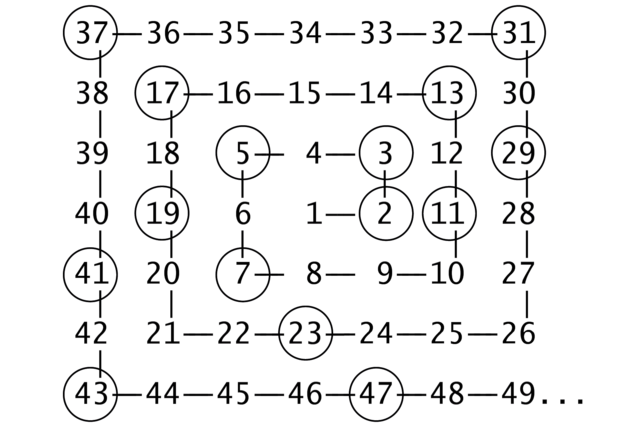
\includegraphics[width = 0.75\linewidth]{Ulam_Spiral.png}
	}
	
	\item Sformułować hipotezę Riemanna.
	\Odp{
		Wszystkie nietrywialne miejsca zerowe funkcji dzeta leża na prostej $\Re z= \frac{1}{2}$
		
		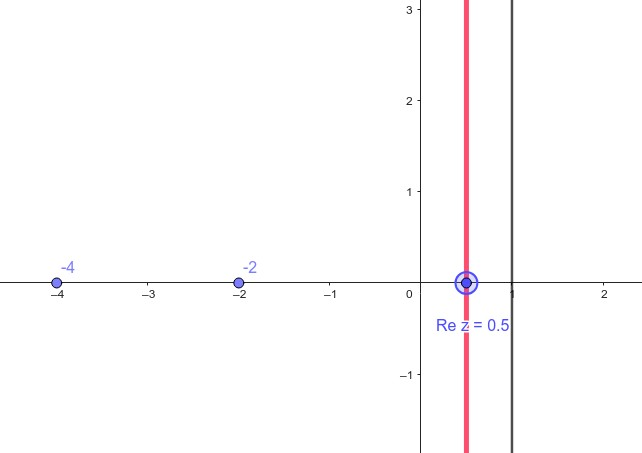
\includegraphics[width=0.75\linewidth]{hpriemanna.jpeg}
		
		Proszę... Tylko bez dowodu...
	}
	
	\item Zdefiniować wielomian (zmiennej rzeczywistej lub zespolonej). Jak nazywają się współczynniki przy najwyższej i najniższej potędze?
	\Odp{
		Wielomianem $n$-tego stopnia nazywamy funkcję
		$$W(z)=a_nz^n+a_{n-1}z^{n-1}+\dots+a_1z^1+a_0,$$
		gdzie $\{a_i\}_{i=1}^n$ to liczby ze zbioru $\mathbb{C}$
	}
	
	\item Wykazać, że wielomian zmiennej rzeczywistej o współczynnikach rzeczywistych stopnia nieparzystego ma zawsze co najmniej jeden pierwiastek rzeczywisty.
	\Odp{
		D: Bez straty ogólności $a_n>0$
		
		$\lim\limits_{x\rightarrow \infty} W(x) = \infty$
		
		$\lim\limits_{x\rightarrow -\infty} W(x) = -\infty$
		
		$\exists_{b_1>0}: W(b_1)>0 \wedge \exists_{b_2<0}: W(b_2)<0$
		
		Z własności Darboux $\exists_{c\in (b_1,b_2)}: W(c)=0$
	}
	
	\item Na wielomiany którego stopnia możemy zawsze rozłożyć wielomian zmiennej rzeczywistej o współczynnikach rzeczywistych?
	\Odp{
		Każdy wielomian o współczynnikach rzeczywistych można rozłożyc na iloczyn wielomianów stopnia co najwyżej 2 o współczynnikach rzeczywistych.
		
		$x^4+1=x^4+2x^2+1-2x^2=(x^2+1)-2x^2 = (x^2-\sqrt{2}x+1)(x^2+\sqrt{2}x+1)$
	}
	
	\item Sformułować zasadnicze twierdzenie algebry.
	\Odp{
		Każdy wielomian o współczynnikach zespolonych $n$-tego stopnia można rozłożyć na iloczym dwumianów o współczynnikach zespolonych (ma dokładnie $n$ pierwiastków zespolonych z krotnościami).
		
		$a_nz^n+\dots+a_1z+a_0=a_n(z-z_1)(z-z_2)\dots(z-z_n)$
	}
	
	\item Podać i udowodnić wzory Viete’a dla trójmianu kwadratowego.
	\Odp{
		$ax^2+bx+c=a(x-x_1)(x-x_2)=ax^2 - a(x_1+x_2)x+ax_1x_2$
		
		$x^2+\frac{b}{a}x+\frac{c}{a}=x^2 - (x_1+x_2) + x_1x_2$
		
		$x_1+x_2 = -\frac{b}{a}\qquad x_1x_2=\frac{c}{a}$
	}
	\newpage
	\item Pokazać mechanizm tworzenia wzorów Viete’a dla wielomianu dowolnego stopnia.
	\Odp{
		Podobnie jak wyżej... (nie będę tego pisał, Ola je udowodniła na ćwiczeniach!)
	}
	
	\item Określić prawdziwość wzorów Viete’a dla trójmianu kwadratowego o współczynnikach rzeczywistych, dla którego wyróżnik $\Delta$ jest ujemny.
	\Odp{
		$x^2+3x+6=0$
		
		$\Delta=-15$
		
		$x_{1,2}=\frac{-1\pm i\sqrt{15}}{2}$
		
		$x_1+x_2 = -3$
		
		$x_1x_2=6$
	}

	\item Podać i udowodnić twierdzenie o podzielności przez $p$ i $q$ odpowiednich współczynników wielomianu o współczynnikach całkowitych, którego liczba wymierna $\frac{p}{q}$ jest pierwiastkiem ($\frac{p}{q}$ jest zapisane w postaci ułamka nieskracalnego).
	\Odp{
		$W(x)=a_nx^n+\dots a_1x+a_0$, $a_i\in\mathbb{Z}$
		
		$\frac{p}{q}$ - pierwiastek wielomianu $\Rightarrow q|a_n$, $p|a_0$
		
		D: $a_n(\frac{p}{q})^n+a_{n-1}(\frac{p}{q})^{n-1}+\dots+a\frac{p}{q}+a_0=0 \quad |\cdot q^n$
		
		$a_np^n+a_{n-1}p^{n-1}q+\dots+a_1pg^{n-1}+a_0q^n=0$
		
		Niech $L=a_np^n+a_{n-1}p^{n-1}q+\dots+a_1pg^{n-1}$, $P=a_{n-1}p^{n-1}q+\dots+a_1pg^{n-1}+a_0q^n$
		
		Wówczas:\\
		
		\begin{tabular}{p{4cm} p{4cm} p{5cm}}
			$p|L$ & $q|P$ &\\
			$p|a_oq^n$ & $q|a_np^n$& ale $p,q$ względnie pierwsze\\
			$p|a_0$&$q|a_n$&\\
		\end{tabular}
		
		
	}
	
	\item Co można powiedzieć o wymiernych pierwiastkach wielomianu $a_nx + \dots + a_1x + a_0,$ którego współczynniki są liczbami całkowitymi? Udowodnić to twierdzenie.
	\Odp{
		To co wyżej.
	}
	
	\item Określić, co (jaki „obiekt”) może być nazywany rozwiązaniem równania czy nierówności.
	\Odp{
		Równianie $\rightarrow$ liczba (pierwiastek) lub zbiór liczb
		
		Nierówność $\rightarrow$ zbiór
	}
	\newpage
	\item Rozwiązywać podstawowe równania i nierówności.
	\Odp{
		\textbf{Zostawiam jako ćwiczenie}
	}
	
	\item Podać podstawowy początek rozwiązywania nierówności typu $\frac{P(x)}{Q(x)} < 0$.
	\Odp{
		Podać dziedzinę oraz pomnożyć obie strony nierówności przez $(Q(x))^2$.
	}
	
	\item Rozwiązywać nierówności pierwiastkowe.
	\Odp{
		\textbf{Zostawiam jako ćwiczenie}
	}
	
	\item Omówić metodę analizy starożytnych stosowaną w równaniach logarytmicznych.
	\Odp{
		Omijamy założenia i rozwiązujemy równanie. Otrzymane rozwiązania podstawiamy i sprawdzamy ich poprawność.
	}
	
	\item Podać schemat rozwiązywania nierówności z wartością bezwzględną.
	\Odp{
		\textbf{Zostawiam jako ćwiczenie}
	}

	\item Rozwiązywać równania (nierówności), w których niewiadoma występuje w postaci	„związanej” (np. w formie $a^x$).
	\Odp{
		\textbf{Zostawiam jako ćwiczenie} ($t=a^x$)
	}
	
	\item Uwalniać ułamki od niewymierności w mianowniku.
	\Odp{
		\textbf{Zostawiam jako ćwiczenie}
	}
	
	\item Wyjaśnić potrzebę uwalniania ułamków od niewymierności w mianowniku.
	\Odp{
		\begin{itemize}
			\item wygląd
			\item oszacowanie (np. możliwość dzielenia na kalkulatorze protstym - a czy Ty wiesz do czego służy MRC, MR+ i MR-?)
			\item odnaleźć się w jakiej strukturze jesteśmy? $\{a+b\sqrt{2} : a,b\in\mathbb{Q}\}$
			\item przygotowanie do działań na $\mathbb{C}$
		\end{itemize}
	}
	\newpage
	\item Podać definicję procentu.
	\Odp{
		Procent jest to sposób zapisu stosunku dwóch wielkości, w którym liczba wyrażona jest jako ułamek o mianowniku 100. Oznaczamy go symoblem $\%$.
	}
	
	\item Wyjaśnić różnicę między procentem a punktem procentowym.
	\Odp{
		\begin{center}
			Procent $\neq$ Punkt procentowy
		\end{center}
		
		Punkt procentowy to różnica między dwoma wartościami procentowymi.
	}
	
	\item Na czym polega błąd definiowania „ignotum per ignotum”?
	\Odp{
		„ignotum per ignotum” - nieznane przez nieznane
		
		Błąd polega w podawaniu obiektu definiowanego jego samego.  
	}
	
	\item Wytłumaczyć schematy definiowania „od ogółu do szczegółu” i z podziałem na klasy równoważności (z przykładami).
	\Odp{
		Zbudowanie hierarchi i stworzenie odpowiedniej struktury.
		
		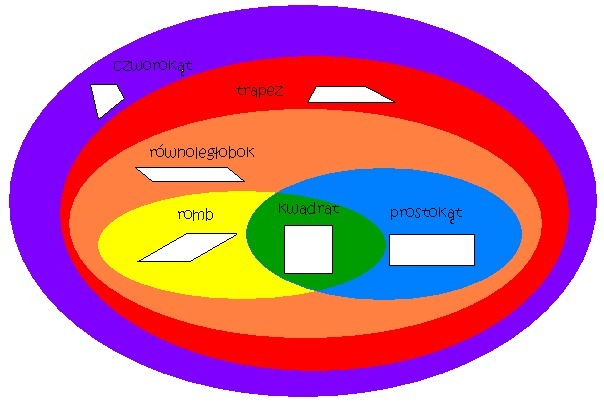
\includegraphics[width=\linewidth]{czwor.jpg}
	}
	\newpage
	\item Podać definicję trapezu i wyjaśnić, dlaczego inne definiowanie nie jest właściwe.
	\Odp{
		Trapez jest to czworokąt, który posiada przynajmniej jedną parę boków równoległych.
		
		Dlaczego inne są niepoprawne?
		\begin{itemize}
			\item psują hierrachie "od ogółu do szczegółu"
			\item definicja powinna działać dla prostokątów, równoległoboków itd.
			\item ma być to klasa domknięta
			\item pojawiają się problemy z pewnymi zadaniami (trapez o największym polu $\rightarrow$ prostokąt)
		\end{itemize}
	}
	
	\item Podać definicję trapezu równoramiennego.
	\Odp{
	Trapez równoramienny to trapez o takich samych kątach przy podstawie \textbf{lub} trapez, który posiada oś symetrii prostopadłą do podstawy.
	}
	
	\item Podać przykłady pokazujące, że czasem pewne obiekty można definiować na różne (istotnie) sposoby, ale nie ma to większego znaczenia, ale czasem ma ogromne znaczenie.
	\Odp{		
		Czy $0\in\mathbb{N}$?\\\\
		
		Ciąg geometryczny
		
		$q=\frac{a_{n+1}}{a_n}$
		
		$2,0,0,0,\dots$ - czy $q=0$? - wszystko jedno\\\\
		
		$\sqrt[3]{a}=b \Leftrightarrow b^3=a$
		
		$\sqrt[3]{a}=b \Leftrightarrow a\geq0,\: b^3=a$\\\\
		
		$\sqrt[n]{a}=b \Leftrightarrow a\geq0,\: b\geq0,\: b^n=a$\\\\
	}
	
	\item Podać „szkolną” definicję prawdopodobieństwa i wyjaśnić, na jakie aspekty należy	przy obliczeniach zwracać szczególną uwagę.
	\Odp{
		$P(A)=\frac{\text{liczba zdarzeń sprzyjających}}{\text{liczba zdarzeń elemetarnych}}$ - przy założeniu jednakowo prawdopodobych zdarzeń
	}
	\newpage
	\item Podać i wyjaśnić paradoks Bertranda.
	\Odp{
		Na okręgu o promieniu 1 wybieramy losowo cieńciwe. Obliczyć prawdopodobieństwo, że jest ona dłuższa niż bok trójkąta równobocznego wpisanego w ten okrąg.
		
		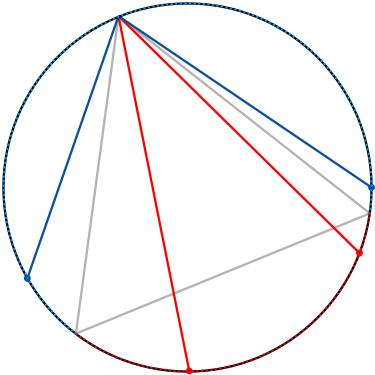
\includegraphics[width=0.33\linewidth]{bertrand1.png}
		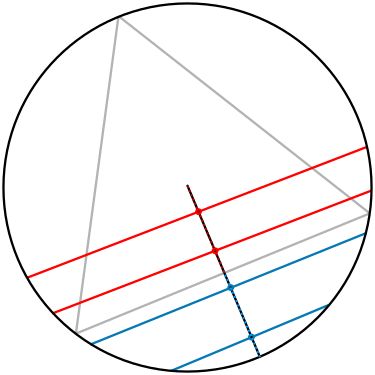
\includegraphics[width=0.33\linewidth]{bertrand2.png}
		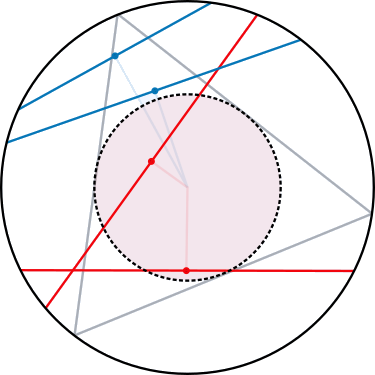
\includegraphics[width=0.33\linewidth]{bertrand3.png}
		
		Prawdopodobieństwa są równe odpowiednio $\frac{1}{3},\frac{1}{2},\frac{1}{4}$. Wszystkie są poprawne i zależą od przyjętej przestrzeni probabilistycznej.
	}
	
	\item Podać definicję Cauchy’ego i definicję Heinego ciągłości funkcji $f : D \rightarrow \mathbb{R}$, przy czym $D \subset R$.
	\Odp{
		\textbf{Definicja Cauchy'ego}
		
		$f:d\rightarrow \mathbb{R}$ ciągła w $x_0 \Leftrightarrow \forall_{\epsilon>0}\exists_{\delta>0}: |x-x_0|<\delta \Rightarrow |f(x)-f(x_0)|<\epsilon$\\\\
		
		\textbf{Definicja Heinego}
		
		$\forall_{(x_n)\subset D} x_n\rightarrow x_0 \Rightarrow f(x_n)\rightarrow f(x)$
		
		
	}
	
	\item Czy funkcja tangens jest ciągła? Odpowiedź uzasadnić.
	\Odp{
		Tak, bo punkty $\{\frac{\pi}{4}+k\pi:k\in\mathbb{Z}\}$ są poza dziedziną funkcji.
	}
	\newpage
	\item Udowodnić równoważność definicji Cauchy’ego i definicję Heinego ciągłości funkcji.
	\Odp{
		D: \textbf{ciągłość Cauchy'ego $\Rightarrow$ ciągłość Heinego}
		
		$(x_n)\subset D, x_n \rightarrow p$
		
		(?) $f(x_n)\rightarrow f(p)$
		
		Ustalmy $\epsilon>0$. Pytamy się, czy $\exists_k n\geq k |f(x_n)-f(p)|<\epsilon$
		
		Z definicji ciągłości Cauchy'ego $\exists_{\delta} |x-p|<
		delta \Rightarrow |f(x)-f(p)|<\epsilon$
		
		Czyli $\exists_k : n\geq k \Rightarrow |x_n-p|<\delta$\\\\
		
		\textbf{ciągłość Heinego $\Rightarrow$ ciągłość Cauchy'ego}
		
		Hp. $\exists_\epsilon : \forall_\delta |x-p|<\delta \not\Rightarrow |f(x)-f(p)|<\epsilon$
		
		Weźmy $\delta = \frac{1}{n}$ z aksjomatu wyboru.
		
		$\forall_{n} \exists_{x_n} : |x_n-p|<\frac{1}{n}, |f(x_n)-f(p)|\geq \epsilon$
		
		$(x_n),x_n\rightarrow p$ $f(x_n)\not\rightarrow f(p)$ sprzeczność
	}
	
	\item Sformułować twierdzenie o własności Darboux oraz twierdzenie Weierstrassa dla funkcji ciągłej $f : [a, b] \rightarrow \mathbb{R}$.
	\Odp{
		\textbf{Własność Darboux}
		
		Z: $f:[a,b]\rightarrow \mathbb{R}$ - ciągła, $f(a)<f(b)$
		
		T: $\forall_{c\in [f(a),f(b)]} \exists_{\xi\in [a,b]} : f(\xi)=c$
		\\\\
		\textbf{Tw Weierstrassa}
		
		Z: $f:[a,b]\rightarrow \mathbb{R}$ - ciągła
		
		T: $\exists_{x_1,x_2 \in [a,b]} \forall_{x\in[a,b]} f(x_1)\leq f(x)\leq f(x_2)$
	}
	
	\item Podać definicję pochodnej funkcji określonej na podzbiorze $D$ zbioru $\mathbb{R}$ o wartościach rzeczywistych w punkcie $x_0 \in D$. Jakie założenie należy uczynić o zbiorze $D$, by można było mówić o pochodnej funkcji?
	\Odp{
		$f:D\rightarrow \mathbb{R}, D\subset \mathbb{R}$ - \underline{otwarty}, $p\in D$
		
		$f'(p)=\lim\limits_{x\rightarrow p} \frac{f(x)-f(p)}{x-p}$
		
		
	}
	
	\item Podać interpretację geometryczną pochodnej.
	\Odp{
		Zobacz: \href{https://tenor.com/view/limite-math-y-axis-x-axis-calculus-gif-14990687}{Fajny gif 1}\hspace{1cm}
		\href{https://tenor.com/view/derivative-gif-23137892}{Fajny gif 2}\hspace{1cm}
		\href{https://tenor.com/view/derivada-gif-22383091}{Fajny gif 3}
	}
	\newpage
	\item Podać warunek konieczny istnienia ekstremum lokalnego funkcji różniczkowalnej.
	\Odp{
		$f$ ma ekstremum lokalne w $x_0$ $\Leftrightarrow f'(x_0)=0$ 
	}
	
	\item Podać warunek wystarczający istnienia maksimum/minimum lokalnego funkcji róż	niczkowalnej (ze zmianą znaku pochodnej) oraz dla funkcji dwukrotnie różniczkowalnej (z drugą pochodną).
	\Odp{
		Warunki wystarczające
		\begin{enumerate}[1)]
			\item $f'(x_0)=0$ oraz zachodzi zmiana znaku pochodnej\\
		
			lub\\
			
			\item $f''(x_0)>0$ dla minimum albo $f''<0$ dla maximum
		\end{enumerate}
	}
	
	\item Sformułować twierdzenie Rolle’a i twierdzenie Lagrange’a.
	\Odp{
		\textbf{Tw Rolle'a}
		
		Z: $f\in C[a,b], f:[a,b]\rightarrow\mathbb{R}$
		
		T: $f(a)=f(b)\Rightarrow \exists_{\xi\in(a,b)}: f'(\xi)=0$\\\\
		
		\textbf{Tw. Lagrange'a}
		
		Z: $f\in C[a,b], f:[a,b]\rightarrow\mathbb{R}$
		
		T: $\exists_{\xi \in (a,b)}: f(\xi)=\frac{f(b)-f(a)}{b-a}$
	}
	
	\item Sformułować regułę de l’Hospitala.
	\Odp{
		$U^*$ - sąsiedztwo $x_0\in\mathbb{R}$. Jeśli spełnione są warunki
		\begin{enumerate}[1)]
			\item $f,g:U^* \rightarrow \mathbb{R}$
			
			$g(x)\neq 0$ dla $x\in U^*$
			
			$g'(x)\neq 0$ dla $x\in U^*$
			
			\item $\lim\limits_{x\rightarrow x_0}f(x)=\lim\limits_{x\rightarrow _0}g(x)=0$
			
			lub
			
			$\lim\limits_{x\rightarrow x_0}f(x)=\lim\limits_{x\rightarrow _0}g(x)=\pm\infty$
			
			\item $\lim\limits_{x\rightarrow x_0} \frac{f'(x)}{g'(x)}=g$
		\end{enumerate}
	
		To: $\lim\limits_{x\rightarrow x_0} \frac{f(x)}{g(x)}=g$
	}
	\newpage
	\item Wytłumaczyć, dlaczego przy korzystaniu z reguły de l’Hospitala nie należy używać skrótu „litera H napisana nad znakiem równości”.
	\Odp{
		A co? Jak się korzysta z właśności Darboux to się pisze literkę "\textbf{D}"?
		
		Co więcej, zapis "$\overset{H}{=}$" oznacza, że obie strony są równe.
	}
	
	\item Wytłumaczyć, dlaczego przy korzystaniu z reguły de l’Hospitala nie należy używać zapisu "$\lim\limits_{x\rightarrow p} \frac{f(x)}{g(x)} \overset{H}{=} \lim\limits_{x\rightarrow p} \frac{f'(x)}{g'(x)}$".
	\Odp{
		Zapis "$\overset{H}{=}$" oznacza, że obie strony są równe.
	}
	
	\item Omówić ryzyko stosowania reguły de l’Hospitala związane z niesprawdzeniem założeń.
	\Odp{
		Przykład: $\lim\limits_{x\rightarrow 0} \frac{\ln (x-2)}{\ln (2-x)}\overset{H}{=}\lim\limits_{x\rightarrow 0}\frac{2-x}{x-2}=-1$
		
		Ale $D=\emptyset$
	}
	
	\item Dlaczego nie można z wykorzystaniem reguły de l’Hospitala liczyć granicy $\lim\limits_{x\rightarrow0}\frac{\sin x}{x}$ ?
	\Odp{
		A skąd znamy pochodną sinusa?
	}
	
	\item Podać fałszywy „dowód” (na podstawie reguły de l’Hospitala) tego, że jeśli funkcja jest różniczkowalna, to jest klasy $C^1$ i pokazać błąd w tym dowodzie.
	\Odp{
		$f$ - różniczkowalna w $[a,b], x_0\in(a,b)$
		
		$f'(x_0)=\lim\limits_{x\rightarrow x_0}\frac{f(x)-f(x_0)}{x-x_0}=\begin{Bmatrix}
			\lim\limits_{x\rightarrow x_0} \frac{f'(x)}{1} = \lim\limits_{x\rightarrow x_0}f'(x)
		\end{Bmatrix}$
	}
	
	\item Wytłumaczyć, dlaczego nie należy robić rzeczy podanych na załączonej „Czarnej liście”.
	\Odp{
	No nie wiem... Czarna lista raczej kojarzy się z rzeczami \textbf{zakazanymi}. Może jednak zasady są po to by je \textbf{przestrzegać} :)
	}
	
	\end{enumerate}
	
\end{document}